\documentclass[10pt]{article}
% Shared preamble: Nature-style article layout (single column, sans headings,
% superscript numbered references, "Fig. 1 |" captions).
\usepackage[a4paper,top=2.2cm,bottom=2.4cm,left=2.4cm,right=2.4cm]{geometry}
\usepackage[T1]{fontenc}
\usepackage[utf8]{inputenc}
\usepackage{newtxtext,newtxmath}
\usepackage[scaled=0.92]{helvet}
\usepackage{microtype}
\usepackage{graphicx}
\usepackage{booktabs,tabularx,multirow,makecell,threeparttable,longtable,array}
\usepackage[table]{xcolor}
\usepackage{siunitx}
\sisetup{group-separator={,},group-minimum-digits=4,detect-all,per-mode=symbol}
\usepackage{amsmath,bm}
\usepackage[version=4]{mhchem}
\usepackage{caption}
\usepackage{titlesec}
\usepackage{enumitem}
\usepackage{fancyhdr}
\usepackage{placeins}
\usepackage{float}
\usepackage{ragged2e}

\definecolor{natureblue}{HTML}{1C5CAB}
\definecolor{inkgray}{HTML}{52514E}

% ---- References: Nature style (biblatex-nature), superscript citations
\usepackage[super,sort&compress,comma]{natbib}
\renewcommand{\bibfont}{\small}
\setlength{\bibsep}{1pt}
\providecommand{\urlprefix}{}
\usepackage{url}

\usepackage[colorlinks=true,linkcolor=natureblue,citecolor=natureblue,
            urlcolor=natureblue,pdfusetitle]{hyperref}

% ---- Headings: bold sans, unnumbered, Nature-like
\titleformat{\section}{\sffamily\bfseries\large}{}{0pt}{}
\titleformat{\subsection}{\sffamily\bfseries\normalsize}{}{0pt}{}
\titleformat{\subsubsection}[runin]{\sffamily\bfseries\normalsize}{}{0pt}{}[.]
\titlespacing*{\section}{0pt}{14pt}{6pt}
\titlespacing*{\subsection}{0pt}{10pt}{3pt}
\titlespacing*{\subsubsection}{0pt}{6pt}{0.6em}
\setcounter{secnumdepth}{0}

% ---- Captions: "Fig. 1 | Title. Legend." in small sans
\DeclareCaptionLabelSeparator{nature}{\,\textbar\,\,}
\captionsetup{font={small,sf},labelfont={bf,sf},labelsep=nature,justification=justified,
              singlelinecheck=false,skip=4pt}
\captionsetup[figure]{name=Fig.}
\captionsetup[table]{name=Table,position=top}

% ---- Misc
\setlength{\parskip}{0pt}
\setlength{\parindent}{1.2em}
\linespread{1.08}
\setlist{nosep,leftmargin=1.4em}
\renewcommand{\arraystretch}{1.12}
\newcommand{\COtwoe}{CO\textsubscript{2}e}
\newcommand{\COtwo}{CO\textsubscript{2}}
\newcommand{\CHfour}{CH\textsubscript{4}}
\newcommand{\NtwoO}{N\textsubscript{2}O}
\newcommand{\figref}[1]{Fig.~\ref{#1}}
\newcommand{\edfigref}[1]{Extended Data Fig.~\ref{#1}}
\newcommand{\edtabref}[1]{Extended Data Table~\ref{#1}}
\newcommand{\sinote}[1]{Supplementary Note~#1}

\pagestyle{fancy}
\fancyhf{}
\renewcommand{\headrulewidth}{0pt}
\fancyfoot[C]{\sffamily\footnotesize\thepage}

% Auto-generated by scripts/run_all.py -- do not edit by hand.
\newcommand{\ArSixDelta}{2.9}
\newcommand{\BasketEqFishDesc}{103\,g lentils, 77\,g kidney beans, 76\,g salmon, 0.5 zinc tablet, 0.2 b12 tablet}
\newcommand{\BasketEqFishEnergy}{1.6}
\newcommand{\BasketEqFishGhg}{1.58}
\newcommand{\BasketEqFishKcal}{374}
\newcommand{\BasketEqFishMass}{256}
\newcommand{\BasketEqFishReduction}{72}
\newcommand{\BasketEqFishShort}{all key nutrients matched}
\newcommand{\BasketEqMeatDesc}{118\,g chickpeas, 54\,g chicken breast, 51\,g lentils, 4\,g mycoprotein, 0.4 zinc tablet, 0.3 b12 tablet}
\newcommand{\BasketEqMeatEnergy}{1.5}
\newcommand{\BasketEqMeatGhg}{0.97}
\newcommand{\BasketEqMeatKcal}{347}
\newcommand{\BasketEqMeatMass}{228}
\newcommand{\BasketEqMeatReduction}{83}
\newcommand{\BasketEqMeatShort}{all key nutrients matched}
\newcommand{\BasketEqVeganDesc}{126\,g kidney beans, 98\,g mycoprotein, 65\,g chickpeas, 0.3 b12 tablet, 0.1 zinc tablet}
\newcommand{\BasketEqVeganEnergy}{1.6}
\newcommand{\BasketEqVeganGhg}{0.36}
\newcommand{\BasketEqVeganKcal}{363}
\newcommand{\BasketEqVeganMass}{290}
\newcommand{\BasketEqVeganReduction}{93}
\newcommand{\BasketEqVeganShort}{all key nutrients matched}
\newcommand{\BasketEqVegetarianDesc}{184\,g kidney beans, 112\,g egg, 0.4 zinc tablet, 0.3 b12 tablet}
\newcommand{\BasketEqVegetarianEnergy}{1.8}
\newcommand{\BasketEqVegetarianGhg}{0.81}
\newcommand{\BasketEqVegetarianKcal}{407}
\newcommand{\BasketEqVegetarianMass}{296}
\newcommand{\BasketEqVegetarianReduction}{86}
\newcommand{\BasketEqVegetarianShort}{all key nutrients matched}
\newcommand{\BasketMeatSwapDesc}{171\,g chicken breast, 85\,g pork loin}
\newcommand{\BasketMeatSwapEnergy}{2.0}
\newcommand{\BasketMeatSwapGhg}{4.02}
\newcommand{\BasketMeatSwapKcal}{460}
\newcommand{\BasketMeatSwapMass}{256}
\newcommand{\BasketMeatSwapReduction}{28}
\newcommand{\BasketMeatSwapShort}{vitamin B\textsubscript{12} short by 57\%}
\newcommand{\BasketOmnivoreDesc}{300\,g milk, 140\,g lentils, 85\,g mycoprotein, 12\,g salmon, 11\,g fortified cereal}
\newcommand{\BasketOmnivoreEnergy}{2.0}
\newcommand{\BasketOmnivoreGhg}{1.59}
\newcommand{\BasketOmnivoreKcal}{460}
\newcommand{\BasketOmnivoreMass}{548}
\newcommand{\BasketOmnivoreReduction}{71}
\newcommand{\BasketOmnivoreShort}{vitamin B\textsubscript{12} short by 23\%}
\newcommand{\BasketVeganFortifiedDesc}{300\,g soy drink, 94\,g mycoprotein, 29\,g pumpkin seeds, 20\,g fortified cereal, 5\,g lentils}
\newcommand{\BasketVeganFortifiedEnergy}{2.0}
\newcommand{\BasketVeganFortifiedGhg}{0.69}
\newcommand{\BasketVeganFortifiedKcal}{460}
\newcommand{\BasketVeganFortifiedMass}{448}
\newcommand{\BasketVeganFortifiedReduction}{88}
\newcommand{\BasketVeganFortifiedShort}{vitamin B\textsubscript{12} short by 54\%}
\newcommand{\BasketVeganWholefoodDesc}{116\,g mycoprotein, 95\,g kidney beans, 81\,g lentils}
\newcommand{\BasketVeganWholefoodEnergy}{1.4}
\newcommand{\BasketVeganWholefoodGhg}{0.38}
\newcommand{\BasketVeganWholefoodKcal}{328}
\newcommand{\BasketVeganWholefoodMass}{292}
\newcommand{\BasketVeganWholefoodReduction}{93}
\newcommand{\BasketVeganWholefoodShort}{vitamin B\textsubscript{12} short by 100\%}
\newcommand{\BasketVegetarianDesc}{300\,g milk, 148\,g lentils, 112\,g soy drink, 84\,g mycoprotein, 3\,g fortified cereal}
\newcommand{\BasketVegetarianEnergy}{2.0}
\newcommand{\BasketVegetarianGhg}{1.46}
\newcommand{\BasketVegetarianKcal}{460}
\newcommand{\BasketVegetarianMass}{646}
\newcommand{\BasketVegetarianReduction}{74}
\newcommand{\BasketVegetarianShort}{vitamin B\textsubscript{12} short by 24\%}
\newcommand{\BeefBtwelve}{2.80}
\newcommand{\BeefBtwelveAbs}{1.68}
\newcommand{\BeefGasChFour}{55}
\newcommand{\BeefGasCoTwo}{24}
\newcommand{\BeefGasNTwoo}{21}
\newcommand{\BeefIron}{3.08}
\newcommand{\BeefIronAbs}{0.61}
\newcommand{\BeefKcal}{230}
\newcommand{\BeefPcKg}{384}
\newcommand{\BeefPcT}{0.38}
\newcommand{\BeefProtein}{28.4}
\newcommand{\BeefProteinQ}{28.1}
\newcommand{\BeefSatfat}{4.7}
\newcommand{\BeefSelenium}{21.6}
\newcommand{\BeefSodium}{87}
\newcommand{\BeefZinc}{6.84}
\newcommand{\BeefZincAbs}{2.39}
\newcommand{\BenefitTotal}{£41k (£21k--68k)}
\newcommand{\BreakEvenLossMeal}{0.52}
\newcommand{\CampusBeefMeals}{79{,}000}
\newcommand{\CampusBeefT}{9.5}
\newcommand{\CampusEfConseq}{31.0}
\newcommand{\CampusLrAcct}{232}
\newcommand{\CampusLrAcctHi}{314}
\newcommand{\CampusLrAcctLo}{165}
\newcommand{\CampusLrGross}{293}
\newcommand{\CampusLrGrossHi}{373}
\newcommand{\CampusLrGrossLo}{233}
\newcommand{\CampusLrLeak}{61}
\newcommand{\CampusLrLeakHi}{109}
\newcommand{\CampusLrLeakLo}{35}
\newcommand{\CampusLrNet}{150}
\newcommand{\CampusLrNetHi}{223}
\newcommand{\CampusLrNetLo}{83}
\newcommand{\CampusLrOff}{17}
\newcommand{\CampusLrOffHi}{51}
\newcommand{\CampusLrOffLo}{3}
\newcommand{\CampusLrSubs}{65}
\newcommand{\CampusLrSubsAdj}{6}
\newcommand{\CampusLrSubsAdjHi}{14}
\newcommand{\CampusLrSubsAdjLo}{0}
\newcommand{\CampusLrSubsHi}{103}
\newcommand{\CampusLrSubsLo}{42}
\newcommand{\CampusNetVsAcctLr}{65}
\newcommand{\CampusNetVsAcctSr}{20}
\newcommand{\CampusNetVsGrossLr}{52}
\newcommand{\CampusNoResponse}{65}
\newcommand{\CampusPassLr}{0.78}
\newcommand{\CampusPassSr}{0.28}
\newcommand{\CampusPctCatering}{7}
\newcommand{\CampusPctImperial}{0.06}
\newcommand{\CampusPeople}{32{,}861}
\newcommand{\CampusPhiStar}{0.25}
\newcommand{\CampusPpmLondon}{5.2}
\newcommand{\CampusProbIncreaseSr}{0.6}
\newcommand{\CampusSrAcct}{233}
\newcommand{\CampusSrAcctHi}{316}
\newcommand{\CampusSrAcctLo}{166}
\newcommand{\CampusSrGross}{294}
\newcommand{\CampusSrGrossHi}{374}
\newcommand{\CampusSrGrossLo}{233}
\newcommand{\CampusSrLeak}{197}
\newcommand{\CampusSrLeakHi}{261}
\newcommand{\CampusSrLeakLo}{148}
\newcommand{\CampusSrNet}{47}
\newcommand{\CampusSrNetHi}{88}
\newcommand{\CampusSrNetLo}{15}
\newcommand{\CampusSrOff}{18}
\newcommand{\CampusSrOffHi}{51}
\newcommand{\CampusSrOffLo}{3}
\newcommand{\CampusSrSubs}{64}
\newcommand{\CampusSrSubsAdj}{36}
\newcommand{\CampusSrSubsAdjHi}{63}
\newcommand{\CampusSrSubsAdjLo}{21}
\newcommand{\CampusSrSubsHi}{103}
\newcommand{\CampusSrSubsLo}{41}
\newcommand{\CarbonValue}{277}
\newcommand{\CarbonValueHigh}{416}
\newcommand{\CarbonValueLow}{139}
\newcommand{\Cbe}{88.0}
\newcommand{\CbeFood}{9.8}
\newcommand{\CocLondonMt}{21}
\newcommand{\CocPerKg}{144}
\newcommand{\CookYield}{0.69}
\newcommand{\CostPerT}{£1{,}730 (£911--3{,}725)}
\newcommand{\CostPerTCapped}{£1{,}444}
\newcommand{\CumGwpHundredFifty}{142}
\newcommand{\CumGwpHundredHundred}{284}
\newcommand{\CumGwpHundredTwenty}{57}
\newcommand{\CumStarFifty}{232}
\newcommand{\CumStarHundred}{308}
\newcommand{\CumStarRatioFifty}{1.6}
\newcommand{\CumStarRatioHundred}{1.1}
\newcommand{\CumStarRatioTwenty}{3.3}
\newcommand{\CumStarTwenty}{186}
\newcommand{\CweKg}{15.8}
\newcommand{\DeltaBtwelveMeal}{1.4}
\newcommand{\DeltaFibreMeal}{3.0}
\newcommand{\DeltaIronAbsMeal}{0.21}
\newcommand{\DeltaIronMeal}{0.42}
\newcommand{\DeltaKcalMeal}{29}
\newcommand{\DeltaPcEqFish}{275}
\newcommand{\DeltaPcEqMeat}{317}
\newcommand{\DeltaPcEqVegan}{359}
\newcommand{\DeltaPcEqVegetarian}{328}
\newcommand{\DeltaProteinMeal}{2.0}
\newcommand{\DeltaZincAbsMeal}{1.08}
\newcommand{\DeltaZincMeal}{2.7}
\newcommand{\DishEps}{1.5}
\newcommand{\EfBeefPnHerd}{99.5}
\newcommand{\EfBeefPnMix}{66.4}
\newcommand{\EfBeefPnUk}{37.1}
\newcommand{\EfBeefUkAttr}{34.7}
\newcommand{\EfBeefUkConseq}{31.0}
\newcommand{\EqBeansAll}{never}
\newcommand{\EqBeansBinding}{vitamin B\textsubscript{12}}
\newcommand{\EqBeansBtwelve}{never}
\newcommand{\EqBeansIron}{207\,g}
\newcommand{\EqBeansProtein}{369\,g}
\newcommand{\EqBeansSelenium}{1.8\,kg}
\newcommand{\EqBeansZinc}{1.2\,kg}
\newcommand{\EqCerealAll}{never}
\newcommand{\EqCerealBinding}{vitamin B6}
\newcommand{\EqCerealBtwelve}{160\,g}
\newcommand{\EqCerealIron}{76\,g}
\newcommand{\EqCerealProtein}{625\,g}
\newcommand{\EqCerealSelenium}{never}
\newcommand{\EqCerealZinc}{383\,g}
\newcommand{\EqCheddarAll}{11.5\,kg}
\newcommand{\EqCheddarBinding}{niacin}
\newcommand{\EqCheddarBtwelve}{235\,g}
\newcommand{\EqCheddarIron}{4.3\,kg}
\newcommand{\EqCheddarProtein}{123\,g}
\newcommand{\EqCheddarSelenium}{76\,g}
\newcommand{\EqCheddarZinc}{188\,g}
\newcommand{\EqChickenAll}{824\,g}
\newcommand{\EqChickenBinding}{vitamin B\textsubscript{12}}
\newcommand{\EqChickenBtwelve}{824\,g}
\newcommand{\EqChickenIron}{349\,g}
\newcommand{\EqChickenProtein}{91\,g}
\newcommand{\EqChickenSelenium}{78\,g}
\newcommand{\EqChickenZinc}{684\,g}
\newcommand{\EqChickpeasAll}{never}
\newcommand{\EqChickpeasBinding}{vitamin B\textsubscript{12}}
\newcommand{\EqChickpeasBtwelve}{never}
\newcommand{\EqChickpeasIron}{210\,g}
\newcommand{\EqChickpeasProtein}{418\,g}
\newcommand{\EqChickpeasSelenium}{584\,g}
\newcommand{\EqChickpeasZinc}{869\,g}
\newcommand{\EqEggAll}{10.6\,kg}
\newcommand{\EqEggBinding}{niacin}
\newcommand{\EqEggBtwelve}{1.7\,kg}
\newcommand{\EqEggIron}{511\,g}
\newcommand{\EqEggProtein}{223\,g}
\newcommand{\EqEggSelenium}{70\,g}
\newcommand{\EqEggZinc}{651\,g}
\newcommand{\EqLentilsAll}{never}
\newcommand{\EqLentilsBinding}{vitamin B\textsubscript{12}}
\newcommand{\EqLentilsBtwelve}{never}
\newcommand{\EqLentilsIron}{183\,g}
\newcommand{\EqLentilsProtein}{537\,g}
\newcommand{\EqLentilsSelenium}{771\,g}
\newcommand{\EqLentilsZinc}{1.0\,kg}
\newcommand{\EqMilkAll}{30.4\,kg}
\newcommand{\EqMilkBinding}{iron}
\newcommand{\EqMilkBtwelve}{488\,g}
\newcommand{\EqMilkIron}{30.4\,kg}
\newcommand{\EqMilkProtein}{852\,g}
\newcommand{\EqMilkSelenium}{864\,g}
\newcommand{\EqMilkZinc}{1.4\,kg}
\newcommand{\EqMycoproteinAll}{never}
\newcommand{\EqMycoproteinBinding}{vitamin B\textsubscript{12}}
\newcommand{\EqMycoproteinBtwelve}{never}
\newcommand{\EqMycoproteinIron}{1.2\,kg}
\newcommand{\EqMycoproteinProtein}{196\,g}
\newcommand{\EqMycoproteinSelenium}{120\,g}
\newcommand{\EqMycoproteinZinc}{137\,g}
\newcommand{\EqOatsAll}{never}
\newcommand{\EqOatsBinding}{vitamin B\textsubscript{12}}
\newcommand{\EqOatsBtwelve}{never}
\newcommand{\EqOatsIron}{143\,g}
\newcommand{\EqOatsProtein}{374\,g}
\newcommand{\EqOatsSelenium}{75\,g}
\newcommand{\EqOatsZinc}{365\,g}
\newcommand{\EqPeaMinceAll}{never}
\newcommand{\EqPeaMinceBinding}{iron}
\newcommand{\EqPeaMinceBtwelve}{never}
\newcommand{\EqPeaMinceIron}{never}
\newcommand{\EqPeaMinceProtein}{241\,g}
\newcommand{\EqPeaMinceSelenium}{never}
\newcommand{\EqPeaMinceZinc}{never}
\newcommand{\EqPeanutsAll}{never}
\newcommand{\EqPeanutsBinding}{vitamin B\textsubscript{12}}
\newcommand{\EqPeanutsBtwelve}{never}
\newcommand{\EqPeanutsIron}{385\,g}
\newcommand{\EqPeanutsProtein}{268\,g}
\newcommand{\EqPeanutsSelenium}{232\,g}
\newcommand{\EqPeanutsZinc}{480\,g}
\newcommand{\EqPeasAll}{never}
\newcommand{\EqPeasBinding}{vitamin B\textsubscript{12}}
\newcommand{\EqPeasBtwelve}{never}
\newcommand{\EqPeasIron}{400\,g}
\newcommand{\EqPeasProtein}{803\,g}
\newcommand{\EqPeasSelenium}{2.2\,kg}
\newcommand{\EqPeasZinc}{2.0\,kg}
\newcommand{\EqPorkAll}{384\,g}
\newcommand{\EqPorkBinding}{vitamin B\textsubscript{12}}
\newcommand{\EqPorkBtwelve}{384\,g}
\newcommand{\EqPorkIron}{306\,g}
\newcommand{\EqPorkProtein}{98\,g}
\newcommand{\EqPorkSelenium}{62\,g}
\newcommand{\EqPorkZinc}{270\,g}
\newcommand{\EqSalmonAll}{1.6\,kg}
\newcommand{\EqSalmonBinding}{zinc}
\newcommand{\EqSalmonBtwelve}{143\,g}
\newcommand{\EqSalmonIron}{1.2\,kg}
\newcommand{\EqSalmonProtein}{127\,g}
\newcommand{\EqSalmonSelenium}{52\,g}
\newcommand{\EqSalmonZinc}{1.6\,kg}
\newcommand{\EqSeedsAll}{never}
\newcommand{\EqSeedsBinding}{vitamin B\textsubscript{12}}
\newcommand{\EqSeedsBtwelve}{never}
\newcommand{\EqSeedsIron}{69\,g}
\newcommand{\EqSeedsProtein}{155\,g}
\newcommand{\EqSeedsSelenium}{230\,g}
\newcommand{\EqSeedsZinc}{170\,g}
\newcommand{\EqSoyDrinkAll}{3.7\,kg}
\newcommand{\EqSoyDrinkBinding}{zinc}
\newcommand{\EqSoyDrinkBtwelve}{884\,g}
\newcommand{\EqSoyDrinkIron}{1.4\,kg}
\newcommand{\EqSoyDrinkProtein}{897\,g}
\newcommand{\EqSoyDrinkSelenium}{939\,g}
\newcommand{\EqSoyDrinkZinc}{3.7\,kg}
\newcommand{\EqTofuAll}{never}
\newcommand{\EqTofuBinding}{vitamin B\textsubscript{12}}
\newcommand{\EqTofuBtwelve}{never}
\newcommand{\EqTofuIron}{229\,g}
\newcommand{\EqTofuProtein}{168\,g}
\newcommand{\EqTofuSelenium}{124\,g}
\newcommand{\EqTofuZinc}{610\,g}
\newcommand{\EqVenisonAll}{210\,g}
\newcommand{\EqVenisonBinding}{selenium}
\newcommand{\EqVenisonBtwelve}{121\,g}
\newcommand{\EqVenisonIron}{92\,g}
\newcommand{\EqVenisonProtein}{106\,g}
\newcommand{\EqVenisonSelenium}{210\,g}
\newcommand{\EqVenisonZinc}{132\,g}
\newcommand{\FlowCwe}{15.8}
\newcommand{\FlowEaten}{6.9}
\newcommand{\FlowEatenGDay}{19}
\newcommand{\FlowRetail}{11.1}
\newcommand{\FoiBeefTwentyFour}{0.07}
\newcommand{\FoiBeefTwentyThree}{8.5}
\newcommand{\FoiBeefTwentyTwo}{10.5}
\newcommand{\FoiChickenTwentyFour}{48.5}
\newcommand{\FoiChickenTwentyThree}{35.8}
\newcommand{\FoiChickenTwentyTwo}{23.8}
\newcommand{\FoiMeatTTwentyFour}{814}
\newcommand{\FoiMeatTTwentyThree}{929}
\newcommand{\FoiMeatTTwentyTwo}{907}
\newcommand{\FoiNarrative}{Beef purchases fell from 10.5\,t (2022/23) and 8.5\,t (2023/24) to 0.07\,t in 2024/25, while venison rose to 1.7\,t and pork and chicken purchases kept growing (to 15.6\,t and at least 48.5\,t). At this study's central emission factors the emissions embodied in meat purchases fell from 929\,t to 814\,t \COtwoe{} despite the growth in volume.}
\newcommand{\FoiPorkTwentyFour}{15.6}
\newcommand{\FoiPorkTwentyThree}{10.3}
\newcommand{\FoiPorkTwentyTwo}{8.3}
\newcommand{\FoiVenisonTwentyFour}{1.7}
\newcommand{\FoiVenisonTwentyThree}{1.6}
\newcommand{\FoiVenisonTwentyTwo}{0.0}
\newcommand{\FreqBtwelve}{27}
\newcommand{\FreqIronWomen}{0.8}
\newcommand{\FreqMeals}{2}
\newcommand{\FreqZincMen}{8}
\newcommand{\FreqZincWomen}{11}
\newcommand{\GwpTwentyDelta}{6.4}
\newcommand{\GwpTwentyFactor}{2.0}
\newcommand{\ImperialStaff}{8{,}941}
\newcommand{\ImperialStudents}{23{,}920}
\newcommand{\ImperialTotalKt}{247}
\newcommand{\Leggi}{28.61}
\newcommand{\LondonBeefMt}{3.49}
\newcommand{\LondonChFourKt}{68}
\newcommand{\LondonConseqDeltaEqFish}{2.13}
\newcommand{\LondonConseqDeltaEqMeat}{2.51}
\newcommand{\LondonConseqDeltaEqVegan}{2.89}
\newcommand{\LondonConseqDeltaEqVegetarian}{2.61}
\newcommand{\LondonDeltaEqFish}{2.50}
\newcommand{\LondonDeltaEqMeat}{2.88}
\newcommand{\LondonDeltaEqVegan}{3.26}
\newcommand{\LondonDeltaEqVegetarian}{2.98}
\newcommand{\LondonDeltaMax}{3.3}
\newcommand{\LondonDeltaMc}{2.8 (2.0--3.7)}
\newcommand{\LondonDeltaMcConseq}{2.4 (1.7--3.2)}
\newcommand{\LondonDeltaMin}{2.5}
\newcommand{\LondonDeltaPnMax}{6.4}
\newcommand{\LondonDeltaPnMin}{5.7}
\newcommand{\LondonPnDeltaEqFish}{5.69}
\newcommand{\LondonPnDeltaEqMeat}{6.07}
\newcommand{\LondonPnDeltaEqVegan}{6.45}
\newcommand{\LondonPnDeltaEqVegetarian}{6.17}
\newcommand{\LpEnergyMaxRatio}{2.0}
\newcommand{\LpEnergyTolHigh}{1.00}
\newcommand{\LpEnergyTolLow}{0.15}
\newcommand{\LpEnergyTolRelaxed}{2.00}
\newcommand{\LpEnergyTolStrict}{0.15}
\newcommand{\LpSatfatMaxRatio}{1.00}
\newcommand{\LpSodiumAllow}{150}
\newcommand{\MealPrice}{6.00}
\newcommand{\MealsM}{1.0}
\newcommand{\MinEnergyEqFish}{1.6}
\newcommand{\MinEnergyEqFishFeasible}{yes}
\newcommand{\MinEnergyEqMeat}{1.2}
\newcommand{\MinEnergyEqMeatFeasible}{yes}
\newcommand{\MinEnergyEqVegan}{1.3}
\newcommand{\MinEnergyEqVeganFeasible}{yes}
\newcommand{\MinEnergyEqVegetarian}{1.6}
\newcommand{\MinEnergyEqVegetarianFeasible}{yes}
\newcommand{\MinEnergyMeatSwap}{2.1}
\newcommand{\MinEnergyMeatSwapFeasible}{no}
\newcommand{\MinEnergyOmnivore}{2.3}
\newcommand{\MinEnergyOmnivoreFeasible}{yes}
\newcommand{\MinEnergyVeganFortified}{5.4}
\newcommand{\MinEnergyVeganFortifiedFeasible}{no}
\newcommand{\MinEnergyVeganWholefood}{1.4}
\newcommand{\MinEnergyVeganWholefoodFeasible}{no}
\newcommand{\MinEnergyVegetarian}{3.8}
\newcommand{\MinEnergyVegetarianFeasible}{no}
\newcommand{\NCampus}{4{,}000}
\newcommand{\NMC}{20{,}000}
\newcommand{\OutsideCost}{3.00}
\newcommand{\PBeefPct}{7.9}
\newcommand{\PaperAuthor}{F.~Song}
\newcommand{\PaperTitle}{Replacing beef: nutrition, emissions and the limits of a campus ban}
\newcommand{\PctCbeConseqEqFish}{2.4}
\newcommand{\PctCbeConseqEqMeat}{2.9}
\newcommand{\PctCbeConseqEqVegan}{3.3}
\newcommand{\PctCbeConseqEqVegetarian}{3.0}
\newcommand{\PctCbeEqFish}{2.8}
\newcommand{\PctCbeEqMeat}{3.3}
\newcommand{\PctCbeEqVegan}{3.7}
\newcommand{\PctCbeEqVegetarian}{3.4}
\newcommand{\PctCbeMax}{3.7}
\newcommand{\PctCbeMin}{2.8}
\newcommand{\PctCbePnEqFish}{6.5}
\newcommand{\PctCbePnEqMeat}{6.9}
\newcommand{\PctCbePnEqVegan}{7.3}
\newcommand{\PctCbePnEqVegetarian}{7.0}
\newcommand{\PctDiet}{16}
\newcommand{\PctLeggiConseqEqFish}{7.4}
\newcommand{\PctLeggiConseqEqMeat}{8.8}
\newcommand{\PctLeggiConseqEqVegan}{10.1}
\newcommand{\PctLeggiConseqEqVegetarian}{9.1}
\newcommand{\PctLeggiEqFish}{8.7}
\newcommand{\PctLeggiEqMeat}{10.1}
\newcommand{\PctLeggiEqVegan}{11.4}
\newcommand{\PctLeggiEqVegetarian}{10.4}
\newcommand{\PctLeggiMax}{11}
\newcommand{\PctLeggiMc}{10\% (7--13\%)}
\newcommand{\PctLeggiMin}{9}
\newcommand{\PctLeggiPnEqFish}{19.9}
\newcommand{\PctLeggiPnEqMeat}{21.2}
\newcommand{\PctLeggiPnEqVegan}{22.5}
\newcommand{\PctLeggiPnEqVegetarian}{21.6}
\newcommand{\PctLeggiPnMax}{23}
\newcommand{\PctLeggiPnMin}{20}
\newcommand{\PctUkCons}{3.1}
\newcommand{\PctUkTerr}{5.9}
\newcommand{\PctVsBeefEqFish}{72}
\newcommand{\PctVsBeefEqMeat}{83}
\newcommand{\PctVsBeefEqVegan}{93}
\newcommand{\PctVsBeefEqVegetarian}{86}
\newcommand{\PerHundredBeefMc}{5.8 (4.7--7.1)}
\newcommand{\PerHundredPnBeefHerd}{16.02}
\newcommand{\PerHundredPnMix}{10.69}
\newcommand{\PerHundredUkAttr}{5.59}
\newcommand{\PerHundredUkConseq}{5.00}
\newcommand{\PopAvgZinc}{0.02}
\newcommand{\PopLondonM}{9.09}
\newcommand{\PopUkM}{69.3}
\newcommand{\PostFarm}{3.0}
\newcommand{\PowerDelta}{0.5}
\newcommand{\PowerN}{770}
\newcommand{\PowerSd}{3.5}
\newcommand{\ProbLossExceeds}{100}
\newcommand{\ReductionMax}{93}
\newcommand{\ReductionMin}{72}
\newcommand{\RetailYield}{0.70}
\newcommand{\TornadoTop}{beef consumption per person}
\newcommand{\UkBeefEnteric}{11.3}
\newcommand{\UkCons}{699.2}
\newcommand{\UkDelta}{22}
\newcommand{\UkTerr}{373.4}
\newcommand{\WasteFrac}{0.10}
\newcommand{\WastePct}{10}
\newcommand{\WelfareAlpha}{0.17}
\newcommand{\WelfareLossCappedTotal}{£214k (£145k--315k)}
\newcommand{\WelfareLossMeal}{£3.25 (£2.09--5.35)}
\newcommand{\WelfareLossMealCapped}{£2.75}
\newcommand{\WelfareLossMealCentral}{3.78}
\newcommand{\WelfareLossTotal}{£254k (£161k--424k)}

\captionsetup[figure]{name=Supplementary Fig.}
\captionsetup[table]{name=Supplementary Table}
\renewcommand{\thetable}{\arabic{table}}
\renewcommand{\thefigure}{\arabic{figure}}
\renewcommand{\theequation}{S\arabic{equation}}
\setcounter{tocdepth}{1}

\begin{document}

\begin{center}
{\sffamily\bfseries\Large Supplementary Information\par}
\vspace{4pt}
{\sffamily\large \PaperTitle\par}
\vspace{6pt}
{\sffamily \PaperAuthor\par}
\end{center}

\noindent This document gives every calculation behind the main paper, step by
step and with the numbers used. All numbers are produced by the code in the
repository (\texttt{scripts/run\_all.py}) and inserted into this document
automatically, so the text, tables and figures cannot drift apart. Central
values are reported first, followed by Monte Carlo medians and 90\% intervals
(5th--95th percentiles) where relevant. Units: kg \COtwoe{} uses
100-year global warming potentials (GWP\textsubscript{100}) unless stated; ``g as
eaten'' means cooked weight for meat, fish and pulses.

{\small\tableofcontents}

%======================================================================
\section{Supplementary Note 1. Imperial College London's beef policy and purchase data}
\label{si:imperial}

\paragraph{Policy timeline.} Imperial's Sustainable Food and Drink Policy
(announced 7 December 2022) committed in-house catering to cut beef by 30\% a
year and to remove it by 2025--26\cite{imperial2022policy}. The College's
own analysis attributed 40\% of catering \COtwoe{} to fresh meat, which was only
8\% of purchases, and 38\% of meat \COtwoe{} to beef\cite{imperial2024beef}.
Taste Imperial removed beef from all of its menus in October
2024\cite{imperial2024beef}. Wild venison was introduced in some dishes, and the
standard meat portion was cut from 120\,g to 100\,g\cite{imperial2026progress}.
The 2026--31 policy binds only in-house kitchens, outlets and events. Outsourced
outlets are encouraged to stop selling beef by 2031\cite{imperial2025policy}.
Imperial College Union's 568 bar stopped serving beef in March 2026\cite{felix2026five}.

\paragraph{Purchase data.} We parsed the line-item food purchase records
released under the Freedom of Information Act (requests IMPFOI-24-576 and
IMPFOI-25-493)\cite{imperialfoi} with \texttt{scripts/foi\_meat\_purchases.py}.
Pack weights were read from free text and multiplied by order quantities.
Lines without a parseable weight were excluded, so the totals are lower bounds.
Supplementary Table~\ref{tab:foi} and Supplementary Fig.~\ref{fig:foi} show the
results.

\begin{table}[H]
\centering\small
\caption{\textbf{Taste Imperial meat purchases (kg product weight per academic year).}
2021/22 is a partial year. Beef was removed in October 2024 (academic year
2024/25). ``Unparsed'' is the number of meat purchase lines without a readable pack
weight. The final columns give the purchases' emissions at this study's central
emission factors (Supplementary Note 5).}
\label{tab:foi}
\begin{tabular}{lrrrrrrrr}
\toprule
Year & Beef (t) & Venison (t) & Lamb (t) & Pork (t) & Chicken (t) & Unparsed & Beef t\COtwoe & All meat t\COtwoe \\
\midrule
2021/22 & 8.26 & 0.00 & 4.2 & 5.6 & 19.3 & 62 & 286 & 713 \\
2022/23 & 10.54 & 0.01 & 5.1 & 8.3 & 23.8 & 50 & 366 & 907 \\
2023/24 & 8.51 & 1.55 & 3.7 & 10.3 & 35.8 & 43 & 295 & 929 \\
2024/25 & 0.07 & 1.68 & 3.4 & 15.6 & 48.5 & 47 & 2 & 814 \\
\bottomrule
\end{tabular}

\end{table}

\begin{figure}[H]
\centering
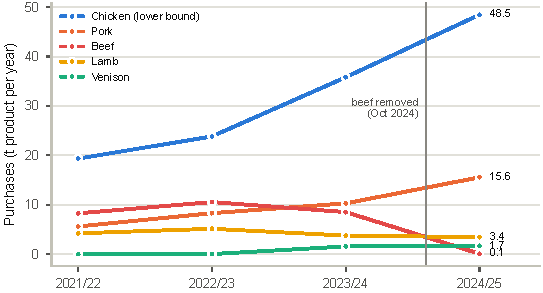
\includegraphics[width=0.62\linewidth]{../figures/si_foi_purchases.pdf}
\caption{\textbf{Meat purchases by Taste Imperial before and after beef removal.}
Lines show kg of product per academic year, from FOI line-item data. Chicken
values are lower bounds. The vertical line marks the removal of beef in
October 2024.}
\label{fig:foi}
\end{figure}

\paragraph{What the purchase data can and cannot show.} \FoiNarrative{}
Chicken purchases were already rising by roughly 12\,t a year before beef was
removed, so a simple before--after comparison would attribute an existing trend
to the policy. Supplementary Note~12 sets out designs that handle this.

%======================================================================
\section{Supplementary Note 2. Food composition and bioavailability}
\label{si:composition}

Nutrient contents $a_{ik}$ of food $i$ and nutrient $k$ are per 100\,g as eaten
(Supplementary Table~\ref{tab:foods}). Beef, the reference food, is lean beef mince
(about 10\% fat), cooked. Four nutrients are adjusted for bioavailability:
\begin{align}
\text{protein}^{q}_{i} &= \text{protein}_i \times \min(\text{DIAAS}_i,\,1), \label{eq:prot}\\
\text{Fe}^{abs}_{i} &= \text{Fe}_i \left[h_i\, a_{\mathrm{haem}} + (1-h_i)\, a_{\mathrm{non\text{-}haem}}\right], \label{eq:fe}\\
\text{Zn}^{abs}_{i} &= \text{Zn}_i\, a_{\mathrm{Zn}}(c_i), \qquad
\text{B}_{12}{}^{abs}_{i} = \text{B}_{12,i}\, a_{\mathrm{B12}}(c_i), \label{eq:zn}
\end{align}
where DIAAS is the digestible indispensable amino acid score\cite{fao2013protein},
$h_i$ the haem fraction of iron, and $a(\cdot)$ the fractional absorption for the
food class $c_i$ (Supplementary Table~\ref{tab:bio}). Truncating DIAAS at 1 counts
only protein that is not limited by its first-limiting indispensable amino acid,
the standard convention for single foods. It ignores complementation between
foods in a mixed basket, so it is conservative for plant baskets.

\begin{table}[H]
\centering\small
\caption{\textbf{Bioavailability parameters.} Central values with the range
used in sensitivity analyses.}
\label{tab:bio}
\begin{tabular}{lcc>{\raggedright\arraybackslash}p{6.3cm}l}
\toprule
Parameter & Central & Range & Note & Ref. \\
\midrule
haem abs & 0.25 & 0.15--0.35 & Haem iron absorption ~25\% (EFSA 2015; FAO/WHO 10-40\%) & \cite{efsa2015iron} \\
nonhaem abs & 0.10 & 0.05--0.15 & Non-haem iron; whole mixed diets 14-18\%, vegetarian 5-12\% & \cite{hurrell2010} \\
zinc abs animal & 0.35 & 0.30--0.40 & Low-phytate diets: FAO/WHO 50/30/15\% at phytate:zinc <5/5-15/>15; IZiNCG 26-34\% mixed diets & \cite{fao2004vitmin} \\
zinc abs mixed & 0.25 & 0.20--0.30 & Moderate-phytate foods (tofu, fortified foods); mycoprotein ileal Zn absorption 24\% (Edwards \& Cummings 2010) & \cite{efsa2014zinc} \\
zinc abs phytate & 0.18 & 0.12--0.25 & Unrefined cereal / legume diets: IZiNCG 18\% (men), 25\% (women) & \cite{izincg2004} \\
zinc abs supplement & 0.40 & 0.30--0.50 & Zinc salts taken with a meal & \cite{efsa2014zinc} \\
b12 abs meat & 0.60 & 0.50--0.70 & Mutton 56-89\%, chicken 61-66\% & \cite{watanabe2007} \\
b12 abs fish & 0.42 & 0.35--0.50 & Trout 42\% & \cite{watanabe2007} \\
b12 abs egg & 0.09 & 0.04--0.20 & Egg B12 poorly absorbed (<9\%) & \cite{watanabe2007} \\
b12 abs dairy & 0.65 & 0.50--0.70 & Milk B12 & \cite{watanabe2007} \\
b12 abs synthetic & 0.50 & 0.40--0.60 & Cyanocobalamin in fortified foods/supplements at low doses & \cite{watanabe2007} \\
\bottomrule
\end{tabular}

\end{table}

\paragraph{Worked example: 100\,g of cooked beef.}
Protein: $28.4\times\min(0.99,1) = 28.1$\,g. Iron: $3.08\times[0.65\times0.25 + 0.35\times0.10] = 0.61$\,mg absorbable. Zinc: $6.84\times0.35 = 2.39$\,mg absorbable. Vitamin B\textsubscript{12}: $2.80\times0.60 = 1.68$\,\textmu g absorbable. These are the targets $b_k$ for the bioavailability-adjusted nutrients; selenium (21.6\,\textmu g) and the other nutrients enter unadjusted.


\begin{table}[p]
\centering\scriptsize
\caption{\textbf{Composition of the reference beef and of the alternative foods, per 100\,g as eaten (one tablet for supplements).}
Sources are given in the last column. ``Diet'' is the food group used to define scenarios.}
\label{tab:foods}
\resizebox{\linewidth}{!}{\begin{tabular}{llrrrrrrrrrrrrrrrrrrll}
\toprule
Food & Diet & kcal & Prot & Fat & SFA & Fib & Fe & Zn & B12 & Nia & B6 & B2 & Se & P & K & Na & Ca & DIAAS & Haem & Zn class & Source \\
\midrule
Beef mince & meat & 230 & 28.4 & 12.0 & 4.7 & 0.0 & 3.08 & 6.84 & 2.80 & 6.8 & 0.43 & 0.19 & 21.6 & 250 & 433 & 87 & 16 & 0.99 & 0.65 & animal & FDC 171794 \\
Chicken breast & meat & 165 & 31.0 & 3.6 & 1.0 & 0.0 & 1.04 & 1.00 & 0.34 & 13.7 & 0.60 & 0.11 & 27.6 & 228 & 256 & 74 & 15 & 1.08 & 0.45 & animal & FDC 171477 \\
Pork loin & meat & 209 & 28.6 & 9.6 & 3.5 & 0.0 & 1.09 & 2.53 & 0.73 & 5.9 & 0.55 & 0.33 & 35.1 & 249 & 425 & 58 & 18 & 1.17 & 0.55 & animal & FDC 168233 \\
Salmon (farmed) & fish & 206 & 22.1 & 12.4 & 2.4 & 0.0 & 0.34 & 0.43 & 2.80 & 8.0 & 0.65 & 0.14 & 41.4 & 252 & 384 & 61 & 15 & 1.00 & 0.35 & animal & FDC 175168 \\
Egg & egg & 155 & 12.6 & 10.6 & 3.3 & 0.0 & 1.19 & 1.05 & 1.11 & 0.1 & 0.12 & 0.51 & 30.8 & 172 & 126 & 124 & 50 & 1.13 & 0.00 & animal & FDC 173424 \\
Cheddar & dairy & 403 & 22.9 & 33.3 & 18.9 & 0.0 & 0.14 & 3.64 & 1.10 & 0.1 & 0.07 & 0.43 & 28.5 & 455 & 76 & 653 & 710 & 1.20 & 0.00 & animal & FDC 173414 \\
Milk & dairy & 50 & 3.3 & 2.0 & 1.3 & 0.0 & 0.02 & 0.48 & 0.53 & 0.1 & 0.04 & 0.18 & 2.5 & 92 & 140 & 47 & 120 & 1.23 & 0.00 & animal & FDC 171267 \\
Tofu & plant & 144 & 17.3 & 8.7 & 1.3 & 2.3 & 2.66 & 1.57 & 0.00 & 0.4 & 0.09 & 0.10 & 17.4 & 190 & 237 & 14 & 683 & 0.97 & 0.00 & mixed & FDC 172475 \\
Lentils & plant & 116 & 9.0 & 0.4 & 0.1 & 7.9 & 3.33 & 1.27 & 0.00 & 1.1 & 0.18 & 0.07 & 2.8 & 180 & 369 & 2 & 19 & 0.58 & 0.00 & phytate & FDC 172421 \\
Chickpeas & plant & 164 & 8.9 & 2.6 & 0.3 & 7.6 & 2.89 & 1.53 & 0.00 & 0.5 & 0.14 & 0.06 & 3.7 & 168 & 291 & 7 & 49 & 0.76 & 0.00 & phytate & FDC 173757 \\
Kidney beans & plant & 127 & 8.7 & 0.5 & 0.1 & 7.4 & 2.94 & 1.07 & 0.00 & 0.6 & 0.12 & 0.06 & 1.2 & 142 & 403 & 2 & 28 & 0.88 & 0.00 & phytate & FDC 175194 \\
Green peas & plant & 78 & 5.2 & 0.3 & 0.0 & 4.5 & 1.52 & 0.67 & 0.00 & 1.5 & 0.11 & 0.10 & 1.0 & 77 & 110 & 72 & 24 & 0.68 & 0.00 & phytate & FDC 170017 \\
Mycoprotein & plant & 98 & 14.5 & 1.7 & 0.4 & 7.2 & 0.50 & 7.00 & 0.00 & 0.0 & 0.00 & 0.00 & 18.0 & 0 & 0 & 50 & 0 & 0.99 & 0.00 & mixed & Quorn labels; Finnigan 2019; Mayer Labba 2022 \\
Pea-protein mince & plant & 196 & 16.0 & 12.0 & 2.9 & 1.2 & 0.00 & 0.00 & 0.00 & 0.0 & 0.00 & 0.00 & 0.0 & 0 & 0 & 300 & 0 & 0.73 & 0.00 & mixed & UK retailer labels \\
Peanuts & plant & 587 & 24.4 & 49.7 & 7.7 & 8.4 & 1.58 & 2.77 & 0.00 & 14.4 & 0.47 & 0.20 & 9.3 & 363 & 634 & 6 & 58 & 0.43 & 0.00 & phytate & FDC 173806 \\
Pumpkin seeds & plant & 559 & 30.2 & 49.0 & 8.7 & 6.0 & 8.82 & 7.81 & 0.00 & 5.0 & 0.14 & 0.15 & 9.4 & 1{,}230 & 809 & 7 & 46 & 0.60 & 0.00 & phytate & FDC 170556 \\
Oats & plant & 379 & 13.2 & 6.5 & 1.1 & 10.1 & 4.25 & 3.64 & 0.00 & 1.1 & 0.10 & 0.15 & 28.9 & 410 & 362 & 6 & 52 & 0.57 & 0.00 & phytate & FDC 173904 \\
Fortified cereal & fortified & 358 & 10.0 & 2.1 & 0.4 & 17.0 & 8.00 & 2.50 & 2.10 & 13.0 & 0.00 & 1.20 & 0.0 & 449 & 533 & 400 & 44 & 0.45 & 0.00 & mixed & UK label (Kellogg's); FDC 173888 \\
Soy drink (fortified) & fortified & 42 & 3.3 & 1.9 & 0.3 & 0.5 & 0.42 & 0.26 & 0.38 & 0.4 & 0.03 & 0.21 & 2.3 & 43 & 122 & 36 & 120 & 0.95 & 0.00 & mixed & UK label (Alpro); FDC 172456 \\
Venison & meat & 187 & 26.4 & 8.2 & 4.0 & 0.0 & 3.35 & 5.20 & 2.32 & 9.3 & 0.47 & 0.33 & 10.3 & 228 & 364 & 78 & 14 & 1.10 & 0.65 & animal & FDC 172603 \\
B12 tablet & supplement & 0 & 0.0 & 0.0 & 0.0 & 0.0 & 0.00 & 0.00 & 10.00 & 0.0 & 0.00 & 0.00 & 0.0 & 0 & 0 & 0 & 0 & 0.00 & 0.00 & animal & assumption \\
Zinc tablet & supplement & 0 & 0.0 & 0.0 & 0.0 & 0.0 & 0.00 & 10.00 & 0.00 & 0.0 & 0.00 & 0.00 & 0.0 & 0 & 0 & 0 & 0 & 0.00 & 0.00 & supplement & assumption \\
\bottomrule
\end{tabular}
}
\end{table}

%======================================================================
\section{Supplementary Note 3. Single-food equivalents}
\label{si:equivalents}

The mass of food $i$ that supplies as much of nutrient $k$ as 100\,g of beef is
\begin{equation}
g_{ik} = 100\,\mathrm{g}\times \frac{b_k}{a_{ik}}, \qquad b_k = a_{\mathrm{beef},k},
\end{equation}
and the mass that matches \emph{every} target nutrient is $g_i = \max_k g_{ik}$.
The nutrient that attains the maximum is the binding nutrient.
Supplementary Table~\ref{tab:equiv} lists $g_{ik}$ for all foods. ``never'' marks a food that
contains none of the nutrient.

\paragraph{Worked example.}
Lentils contain $9.02\times0.58 = 5.23$\,g quality-adjusted protein per 100\,g, so matching beef's 28.1\,g needs $100\times28.1/5.23 = 537$\,g. Their 1.27\,mg zinc is absorbed at 0.18 ($0.229$\,mg), so matching beef's 2.39\,mg absorbable zinc needs 1{,}047\,g. Lentils contain no vitamin B\textsubscript{12}, so no amount of lentils matches every nutrient (``never''). Chicken breast, by contrast, matches protein with 91\,g but needs 684\,g for zinc and 824\,g for vitamin B\textsubscript{12}.


\begin{table}[p]
\centering\scriptsize
\caption{\textbf{Grams of each food (as eaten) that supply the nutrient content of 100\,g cooked beef.}
Protein, iron, zinc and vitamin B\textsubscript{12} are bioavailability-adjusted.
The last two columns give the amount needed to match all ten nutrients and the
binding nutrient. Values above 2,000\,g are shown as ``>2k''.}
\label{tab:equiv}
\resizebox{\linewidth}{!}{\begin{tabular}{lrrrrrrrrrrrl}
\toprule
Food & Prot.* & Fe* & Zn* & B12* & Nia & B6 & B2 & Se & P & K & All & Binding \\
\midrule
Venison & 106 & 92 & 132 & 121 & 73 & 91 & 58 & 210 & 110 & 119 & 210 & Selenium \\
Pork loin & 98 & 306 & 270 & 384 & 115 & 78 & 58 & 62 & 100 & 102 & 384 & B\textsubscript{12} (absorbable) \\
Chicken breast & 91 & 349 & 684 & 824 & 50 & 71 & 168 & 78 & 110 & 169 & 824 & B\textsubscript{12} (absorbable) \\
Salmon (farmed) & 127 & 1{,}173 & 1{,}591 & 143 & 85 & 66 & 141 & 52 & 99 & 113 & 1{,}591 & Zinc (absorbable) \\
Soy drink (fortified) & 897 & 1{,}448 & >2k & 884 & 1{,}600 & 1{,}381 & 91 & 939 & 581 & 355 & >2k & Zinc (absorbable) \\
Egg & 223 & 511 & 651 & 1{,}682 & >2k & 354 & 37 & 70 & 145 & 344 & >2k & Niacin \\
Cheddar & 123 & >2k & 188 & 235 & >2k & 648 & 45 & 76 & 55 & 570 & >2k & Niacin \\
Milk & 852 & >2k & 1{,}425 & 488 & >2k & 1{,}126 & 103 & 864 & 272 & 309 & >2k & Iron (absorbable) \\
Tofu & 168 & 229 & 610 & never & 1{,}785 & 465 & 187 & 124 & 132 & 183 & never & B\textsubscript{12} (absorbable) \\
Lentils & 537 & 183 & 1{,}047 & never & 642 & 240 & 262 & 771 & 139 & 117 & never & B\textsubscript{12} (absorbable) \\
Chickpeas & 418 & 210 & 869 & never & 1{,}293 & 308 & 303 & 584 & 149 & 149 & never & B\textsubscript{12} (absorbable) \\
Green peas & 803 & 400 & 1{,}985 & never & 459 & 379 & 191 & >2k & 325 & 394 & never & B\textsubscript{12} (absorbable) \\
Mycoprotein & 196 & 1{,}217 & 137 & never & never & never & never & 120 & never & never & never & B\textsubscript{12} (absorbable) \\
Pea-protein mince & 241 & never & never & never & never & never & never & never & never & never & never & Iron (absorbable) \\
Peanuts & 268 & 385 & 480 & never & 47 & 92 & 97 & 232 & 69 & 68 & never & B\textsubscript{12} (absorbable) \\
Pumpkin seeds & 155 & 69 & 170 & never & 136 & 299 & 125 & 230 & 20 & 54 & never & B\textsubscript{12} (absorbable) \\
Oats & 374 & 143 & 365 & never & 607 & 428 & 123 & 75 & 61 & 120 & never & B\textsubscript{12} (absorbable) \\
Fortified cereal & 625 & 76 & 383 & 160 & 52 & never & 16 & never & 56 & 81 & never & Vitamin B6 \\
Kidney beans & 369 & 207 & 1{,}243 & never & 1{,}176 & 357 & 329 & 1{,}800 & 176 & 107 & never & B\textsubscript{12} (absorbable) \\
\bottomrule
\end{tabular}
}
\end{table}

%======================================================================
\section{Supplementary Note 4. Nutrient-matching linear programmes}
\label{si:lp}

For a set $A$ of allowed foods, the basket $x_i\ge 0$ (units of 100\,g as eaten, or
tablets) that replaces 100\,g of beef solves
\begin{align}
\min_{x,\,s}\;& \sum_{i\in A} c_i x_i + M\sum_{k} s_k \\
\text{s.t.}\;& \sum_{i\in A} \frac{a_{ik}}{b_k}\,x_i + s_k \ge 1 \quad \forall k \in K, \qquad 0\le s_k\le 1,\\
& (1-\delta_{\mathrm{lo}})\,E_{\mathrm{beef}} \le \sum_i e_i x_i \le (1+\delta_{\mathrm{hi}})\,E_{\mathrm{beef}},\\
& \sum_i \mathrm{SFA}_i\, x_i \le \rho\,\mathrm{SFA}_{\mathrm{beef}}, \qquad
\sum_i \mathrm{Na}_i\, x_i \le \mathrm{Na}_{\mathrm{beef}} + \Delta_{\mathrm{Na}},\\
& 0 \le x_i \le \bar{x}_i ,
\end{align}
where $K$ is the set of ten target nutrients (bioavailability-adjusted protein,
iron, zinc and vitamin B\textsubscript{12}, plus niacin, vitamin B\textsubscript{6},
riboflavin, selenium, phosphorus and potassium), $c_i$ the emissions per unit
(minimum-GHG objective) or the mass per unit (minimum-mass objective), $e_i$
energy, and $\bar{x}_i$ a portion cap. Settings: energy band
$\delta_{\mathrm{lo}}=\LpEnergyTolLow$, $\delta_{\mathrm{hi}}=\LpEnergyTolHigh$
(relaxed to $\LpEnergyTolRelaxed$ in sensitivity analysis); saturated fat ratio
$\rho=\LpSatfatMaxRatio$; extra sodium allowance $\Delta_{\mathrm{Na}}=\LpSodiumAllow$\,mg;
portion caps in Supplementary Table~\ref{tab:foods}. The shortfall slacks $s_k$ carry a penalty
$M=100$\,kg \COtwoe{} per unit of fractional shortfall. Any basket's emissions are
below 1\,kg \COtwoe{}, so the slacks are used only when no feasible basket
exists, and they then report the unavoidable shortfall. The programmes are
solved with HiGHS through \texttt{scipy.optimize.linprog}.

Scenarios restrict $A$ by food group: omnivore without ruminant meat
(poultry, pork, fish, eggs, dairy, plants, fortified foods); poultry and pork only;
pescatarian; vegetarian; vegan with fortified foods; vegan with fortified foods
and supplements; and vegan from whole foods only. Supplementary Table~\ref{tab:baskets}
gives the solutions and Supplementary Table~\ref{tab:basketsens} the sensitivity analyses.

\begin{table}[p]
\centering\scriptsize
\caption{\textbf{Optimised baskets replacing 100\,g of cooked beef.} Composition in g as
eaten (supplements in tablets), emissions with central emission factors, and
the supply of each target nutrient relative to beef (1.00 = equal).}
\label{tab:baskets}
\resizebox{\linewidth}{!}{\begin{tabular}{>{\raggedright\arraybackslash}p{2.2cm}>{\raggedright\arraybackslash}p{4.6cm}rrrrrrrrrrrrrc}
\toprule
Scenario & Composition per 100\,g beef replaced & kg\,\COtwoe & g & kcal ratio & Prot.* & Fe* & Zn* & B12* & Nia & B6 & B2 & Se & P & K & Key matched \\
\midrule
Poultry \& pork only & 171\,g chicken breast, 85\,g pork loin & 4.02 & 256 & 2.00 & 2.75 & 0.77 & 0.56 & 0.43 & 4.19 & 3.50 & 2.48 & 3.57 & 2.41 & 1.85 & no \\
Omnivore, foods only & 300\,g milk, 140\,g lentils, 85\,g mycoprotein, 12\,g salmon, 11\,g fortified cereal & 1.59 & 548 & 2.00 & 1.16 & 1.00 & 1.00 & 0.77 & 0.61 & 1.04 & 4.21 & 1.47 & 2.43 & 2.41 & no \\
Vegetarian, foods only & 300\,g milk, 148\,g lentils, 112\,g soy drink, 84\,g mycoprotein, 3\,g fortified cereal & 1.46 & 646 & 2.00 & 1.18 & 1.00 & 1.00 & 0.76 & 0.39 & 0.96 & 4.87 & 1.35 & 2.41 & 2.58 & no \\
Vegan incl. fortified foods & 300\,g soy drink, 94\,g mycoprotein, 29\,g pumpkin seeds, 20\,g fortified cereal, 5\,g lentils & 0.69 & 448 & 2.00 & 1.05 & 1.00 & 1.00 & 0.46 & 0.79 & 0.34 & 4.80 & 1.24 & 2.36 & 1.68 & no \\
Vegan, whole foods only & 116\,g mycoprotein, 95\,g kidney beans, 81\,g lentils & 0.38 & 292 & 1.43 & 1.00 & 1.00 & 1.00 & 0.00 & 0.21 & 0.61 & 0.60 & 1.12 & 1.13 & 1.58 & no \\
\midrule
Poultry/pork-led & 118\,g chickpeas, 54\,g chicken breast, 51\,g lentils, 4\,g mycoprotein, 0.4 zinc tablet, 0.3 b12 tablet & 0.97 & 228 & 1.51 & 1.00 & 1.00 & 1.00 & 1.00 & 1.27 & 1.36 & 0.91 & 1.00 & 1.66 & 1.55 & yes \\
Fish-led & 103\,g lentils, 77\,g kidney beans, 76\,g salmon, 0.5 zinc tablet, 0.2 b12 tablet & 1.58 & 256 & 1.63 & 1.00 & 1.00 & 1.00 & 1.00 & 1.13 & 1.80 & 1.17 & 1.64 & 1.95 & 2.27 & yes \\
Dairy/egg-led & 184\,g kidney beans, 112\,g egg, 0.4 zinc tablet, 0.3 b12 tablet & 0.81 & 296 & 1.77 & 1.00 & 1.11 & 1.00 & 1.00 & 0.17 & 0.83 & 3.56 & 1.69 & 1.81 & 2.04 & yes \\
Plant-based & 126\,g kidney beans, 98\,g mycoprotein, 65\,g chickpeas, 0.3 b12 tablet, 0.1 zinc tablet & 0.36 & 290 & 1.58 & 1.00 & 1.00 & 1.00 & 1.00 & 0.16 & 0.57 & 0.60 & 1.00 & 1.15 & 1.61 & yes \\
\bottomrule
\end{tabular}
}
\end{table}

\begin{table}[H]
\centering\small
\caption{\textbf{Sensitivity of basket emissions (kg \COtwoe{} per 100\,g beef replaced) and mass (g) to bioavailability and energy assumptions.}
Infeasible baskets (shortfall in at least one nutrient) are marked with~$^\dagger$.}
\label{tab:basketsens}
\resizebox{\linewidth}{!}{\begin{tabular}{lrrrrrrr}
\toprule
Scenario & Central & No bioavail. adj. & Plant-unfavourable & Plant-favourable & Energy $\pm$15\% & Energy $\le$3$\times$ & All ten nutrients \\
\midrule
Poultry \& pork only & 4.02 / 256$^\dagger$ & 4.02 / 256$^\dagger$ & 4.02 / 256$^\dagger$ & 4.02 / 256$^\dagger$ & 2.16 / 127$^\dagger$ & 4.31 / 277$^\dagger$ & 4.02 / 256$^\dagger$ \\
Omnivore, foods only & 1.59 / 548$^\dagger$ & 1.43 / 439 & 3.00 / 360$^\dagger$ & 1.54 / 447 & 0.79 / 178$^\dagger$ & 2.25 / 654 & 1.64 / 446$^\dagger$ \\
Vegetarian, foods only & 1.46 / 646$^\dagger$ & 1.47 / 699$^\dagger$ & 1.45 / 576$^\dagger$ & 1.30 / 684$^\dagger$ & 0.60 / 438$^\dagger$ & 1.61 / 872$^\dagger$ & 1.13 / 455$^\dagger$ \\
Vegan incl. fortified foods & 0.69 / 448$^\dagger$ & 0.62 / 410$^\dagger$ & 0.55 / 344$^\dagger$ & 0.67 / 462$^\dagger$ & 0.60 / 438$^\dagger$ & 0.79 / 635$^\dagger$ & 0.55 / 421$^\dagger$ \\
Vegan, whole foods only & 0.38 / 292$^\dagger$ & 0.32 / 274$^\dagger$ & 0.54 / 422$^\dagger$ & 0.36 / 272$^\dagger$ & 0.46 / 236$^\dagger$ & 0.38 / 292$^\dagger$ & 0.59 / 395$^\dagger$ \\
\midrule
Poultry/pork-led & 0.97 / 228 & 0.80 / 202 & 1.36 / 361$^\dagger$ & 0.96 / 175 & 1.13 / 199$^\dagger$ & 0.97 / 228 & 0.97 / 226 \\
Fish-led & 1.58 / 256 & 1.24 / 183 & 1.65 / 294$^\dagger$ & 1.56 / 224 & 1.05 / 189$^\dagger$ & 1.58 / 256 & 1.58 / 256 \\
Dairy/egg-led & 0.81 / 296 & 0.64 / 282 & 0.87 / 356$^\dagger$ & 0.81 / 296 & 0.47 / 208$^\dagger$ & 0.81 / 296 & 0.82 / 291$^\dagger$ \\
Plant-based & 0.36 / 290 & 0.32 / 274 & 0.51 / 373$^\dagger$ & 0.36 / 272 & 0.58 / 190$^\dagger$ & 0.36 / 290 & 0.59 / 409 \\
\bottomrule
\end{tabular}
}
\end{table}

%======================================================================
\section{Supplementary Note 5. Emission factors and the UK beef supply mix}
\label{si:ef}

\paragraph{Alternative foods.} Emission factors (EFs) are kg \COtwoe{} per kg as
purchased, cradle to retail (Supplementary Table~\ref{tab:efs}). The central values are UK- or
Europe-relevant where available, with Poore \& Nemecek's global means\cite{poore2018}
as a comparison. Emissions per LP unit as eaten are
\begin{equation}
\mathrm{GHG}_i = \frac{m_i}{y_i\,(1-w)}\;\mathrm{EF}_i,
\end{equation}
with unit mass $m_i=0.1$\,kg, cooking yield $y_i$ (kg as eaten per kg purchased),
and household waste fraction $w=\WasteFrac$ applied equally to all foods.

\begin{table}[p]
\centering\scriptsize
\caption{\textbf{Emission factors (kg \COtwoe{} per kg as purchased).} Central value, 90\% interval used
in Monte Carlo sampling (log-normal), Poore \& Nemecek global mean, cooking yield and greenhouse-gas
composition used for metric conversions.}
\label{tab:efs}
\resizebox{\linewidth}{!}{\begin{tabular}{lrrrrrlll}
\toprule
Food & Central & Median & 5th--95th & P\&N mean & Yield & CO$_2$/CH$_4$/N$_2$O & GWP & Note \\
\midrule
beef mince & 34.70 & 34.70 & 24.00--52.00 & 66.39 & 0.69 & 0.20/0.58/0.22 & AR5 & UK supply mix (overridden in model); ef\_pn = 50:50 beef/dairy herd \\
chicken breast & 9.87 & 7.52 & 3.95--20.82 & 9.87 & 0.73 & 0.61/0.06/0.33 & AR5cc & Poultry meat \\
pork loin & 12.31 & 10.57 & 6.91--23.79 & 12.31 & 0.80 & 0.49/0.25/0.26 & AR5cc & Pig meat \\
salmon & 13.63 & 7.89 & 5.41--32.64 & 13.63 & 0.80 & 0.70/0.10/0.20 & AR5cc & Fish (farmed) \\
egg & 4.67 & 4.21 & 2.85--8.49 & 4.67 & 0.88 & 0.55/0.10/0.35 & AR5cc & Eggs; cook\_yield = edible share of shell egg \\
cheddar & 23.88 & 18.64 & 10.21--58.79 & 23.88 & 1.00 & 0.30/0.50/0.20 & AR5cc & Cheese \\
milk & 3.15 & 2.65 & 1.51--7.00 & 3.15 & 1.00 & 0.30/0.50/0.20 & AR5cc & Milk \\
tofu & 3.16 & 2.58 & 1.41--7.27 & 3.16 & 1.00 & 0.65/0.05/0.30 & AR5cc & Tofu \\
lentils & 1.79 & 1.39 & 0.89--4.00 & 1.79 & 2.73 & 0.65/0.05/0.30 & AR5cc & Other pulses (dry weight) \\
chickpeas & 1.79 & 1.39 & 0.89--4.00 & 1.79 & 2.31 & 0.65/0.05/0.30 & AR5cc & Other pulses (dry weight) \\
kidney beans & 1.79 & 1.39 & 0.89--4.00 & 1.79 & 2.50 & 0.65/0.05/0.30 & AR5cc & Other pulses (dry weight) \\
peas & 0.98 & 0.80 & 0.51--1.87 & 0.98 & 0.89 & 0.65/0.05/0.30 & AR5cc & Peas \\
mycoprotein & 1.89 & 1.89 & 1.26--2.60 & -- & 1.00 & 0.80/0.05/0.15 & AR5 & Quorn Mince farm-to-shop (Carbon Trust / ClimatePartner verified) \\
pea mince & 2.00 & 2.00 & 0.90--4.00 & -- & 0.90 & 0.75/0.05/0.20 & AR5 & Plant-based mince; 0.75-0.98 factory gate (GFI) to 3.2-3.5 (Beyond/Impossible) \\
peanuts & 3.23 & 3.29 & 1.42--6.15 & 3.23 & 1.00 & 0.65/0.05/0.30 & AR5cc & Groundnuts \\
pumpkin seeds & 3.23 & 3.29 & 1.42--6.15 & -- & 1.00 & 0.65/0.05/0.30 & AR5cc & Proxy: groundnuts (no seed LCA in P\&N) \\
oats & 2.48 & 2.59 & 0.80--4.30 & 2.48 & 1.00 & 0.65/0.05/0.30 & AR5cc & Oatmeal (dry weight) \\
fortified cereal & 2.36 & 1.91 & 1.07--4.61 & -- & 1.00 & 0.70/0.05/0.25 & AR5cc & Proxy: P\&N wheat (bread) x 1.5 for processing and packaging \\
soy drink & 0.98 & 0.91 & 0.51--1.74 & 0.98 & 1.00 & 0.65/0.05/0.30 & AR5cc & Soymilk (per kg ~ per L) \\
venison & 3.00 & 3.00 & 1.00--12.00 & -- & 0.83 & 1.00/0.00/0.00 & AR5 & Wild-shot deer: processing and transport only (assumption; Imperial cites <1/3 of beef) \\
lamb & 39.72 & 40.61 & 23.70--60.16 & 39.72 & 0.72 & 0.20/0.55/0.25 & AR5cc & Lamb \& mutton (EDM cross-effects only) \\
b12 supplement & 50.00 & 50.00 & 20.00--100.00 & -- & 1.00 & 1.00/0.00/0.00 & AR5 & Per kg of tablets (one tablet ~0.1 g) \\
zinc supplement & 50.00 & 50.00 & 20.00--100.00 & -- & 1.00 & 1.00/0.00/0.00 & AR5 & Per kg of tablets (one tablet ~0.1 g) \\
\bottomrule
\end{tabular}
}
\end{table}

\paragraph{Beef consumed in the UK.} The EF of beef is built from the origin
and production-system mix of UK beef consumption (Supplementary Table~\ref{tab:beefmix}).
Farm-gate footprints per kg carcass weight equivalent (cwe) are converted to
retail boneless meat and given a post-farm-gate adder:
\begin{equation}
\mathrm{EF}^{\mathrm{retail}}_{j} = \frac{\mathrm{EF}^{\mathrm{farm}}_{j}}{r} + p,
\qquad \mathrm{EF}_{\mathrm{beef}} = \sum_j s_j\,\mathrm{EF}^{\mathrm{retail}}_j,
\end{equation}
where $r=\RetailYield$ is the carcass-to-retail yield, $p=\PostFarm$\,kg \COtwoe{}\,kg$^{-1}$
the post-farm-gate emissions, and $s_j$ the market share of segment $j$. The
\emph{consequential} variant multiplies each farm-gate EF by an avoidable
fraction $f_j$. Beef from the dairy herd is a co-product of milk. If its beef is
no longer demanded, the cow's emissions are reallocated to milk rather than
avoided, so only the calf-rearing and finishing emissions disappear.

\begin{table}[H]
\centering\small
\caption{\textbf{UK beef supply mix.} Shares of consumption, farm-gate footprints and the resulting retail EFs.}
\label{tab:beefmix}
\resizebox{\linewidth}{!}{\begin{tabular}{lrrrrrrl}
\toprule
Segment & Share & Farm EF (cwe) & 90\% range & Retail EF & Avoidable & Retail EF (conseq.) & Ref. \\
\midrule
UK suckler herd & 0.360 & 28.0 & 20--38 & 43.0 & 1.00 & 43.0 & \cite{ciel2020,prism2024} \\
UK dairy-origin & 0.360 & 16.0 & 10--24 & 25.9 & 0.70 & 19.0 & \cite{ciel2020,prism2024} \\
Ireland & 0.216 & 20.0 & 14--30 & 31.6 & 0.85 & 27.3 & \cite{gerber2013,bordbia2024} \\
Other Europe & 0.035 & 22.0 & 14--35 & 34.4 & 0.75 & 26.6 & \cite{gerber2013} \\
Australia \& New Zealand & 0.015 & 25.0 & 15--45 & 38.7 & 1.00 & 38.7 & \cite{gerber2013} \\
South America & 0.015 & 60.0 & 30--150 & 88.7 & 1.00 & 88.7 & \cite{gerber2013,poore2018} \\
\midrule
\textbf{UK consumption mix} & 1.001 &  &  & \textbf{34.7} &  & \textbf{31.0} &  \\
\bottomrule
\end{tabular}
}
\end{table}

\paragraph{Worked calculation.}
For the UK suckler herd: $28.0/0.70 + 3.0 = 43.0$\,kg \COtwoe{} per kg retail beef. Weighting all six segments by their shares gives $\mathrm{EF}_{\mathrm{beef}} = 34.7$\,kg \COtwoe\,kg$^{-1}$ (attributional) and 31.0\,kg \COtwoe\,kg$^{-1}$ (consequential). For comparison, Poore \& Nemecek's global means are 99.48 (beef herd) and 33.30 (dairy herd), 66.4 for a 50:50 mix, and their UK producers average 48.4 and 25.9 (mix 37.1), close to our bottom-up estimate. Per 100\,g cooked beef: $34.7\times 0.1/(0.69\times0.90) = 5.59$\,kg \COtwoe.


%======================================================================
\section{Supplementary Note 6. From one portion to London and the UK}
\label{si:scaling}

Per-capita beef flows follow the supply chain from the national supply balance:
\begin{align}
B_{\mathrm{retail}} &= B_{\mathrm{cwe}}\, r, \qquad
B_{\mathrm{eaten}} = B_{\mathrm{retail}}\,(1-w)\, y_{\mathrm{beef}},
\end{align}
where $B_{\mathrm{cwe}}$ is beef consumption in carcass-weight equivalent per person per year,
$r$ the retail yield, $w$ household waste and $y_{\mathrm{beef}}$ the cooking yield.
The annual change in emissions per person when beef is replaced by basket $b$ is
\begin{equation}
\Delta e = \underbrace{10\,B_{\mathrm{eaten}}\;\mathrm{GHG}_b}_{\text{replacement}}
- \underbrace{B_{\mathrm{retail}}\;\mathrm{EF}_{\mathrm{beef}}}_{\text{beef}},
\end{equation}
with $\mathrm{GHG}_b$ in kg \COtwoe{} per 100\,g of beef replaced (hence the factor 10
per kg). London and UK totals multiply by population.

\paragraph{Worked calculation (central values, omnivore basket).}
Beef supply is $B_{\mathrm{cwe}}=15.8$\,kg per person per year, i.e. $B_{\mathrm{retail}} = 15.8\times0.70 = 11.06$\,kg bought and $B_{\mathrm{eaten}} = 11.06\times0.90\times0.69 = 6.87$\,kg cooked beef eaten (19\,g a day). Beef emissions per person are $11.06\times34.7 = 384$\,kg \COtwoe{} a year. The poultry/pork-led basket emits 0.969\,kg \COtwoe{} per 100\,g beef replaced, so the replacement emits $10\times6.87\times0.969 = 67$\,kg. The change is $\textminus 317$\,kg per person (\textminus 83\% of beef's footprint). Multiplying by 9{,}089{,}736 Londoners gives $\textminus 2.88$\,Mt \COtwoe{} a year, i.e. 10.1\% of London's territorial emissions (28.61\,Mt) and 3.3\% of its consumption-based emissions (88.0\,Mt).


\begin{table}[H]
\centering\small
\caption{\textbf{Annual emissions change from replacing all beef eaten by Londoners with nutritionally equivalent baskets.}
Central values. Percentages are relative to London's territorial emissions
(LEGGI 2023) and to London's consumption-based emissions.}
\label{tab:scaling}
\resizebox{\linewidth}{!}{\begin{tabular}{llrrrrrrrrr}
\toprule
Beef EF & Basket & Beef kg/p & Alt. kg/p & \% vs beef & London beef Mt & $\Delta$ London Mt & \% LEGGI & \% CBE & $\Delta$ UK Mt & \% UK terr. \\
\midrule
UK mix & Poultry/pork-led & 384 & 67 & \textminus 83 & 3.49 & \textminus 2.88 & \textminus 10.1 & \textminus 3.3 & \textminus 22.0 & \textminus 5.9 \\
UK mix & Fish-led & 384 & 109 & \textminus 72 & 3.49 & \textminus 2.50 & \textminus 8.7 & \textminus 2.8 & \textminus 19.0 & \textminus 5.1 \\
UK mix & Dairy/egg-led & 384 & 56 & \textminus 86 & 3.49 & \textminus 2.98 & \textminus 10.4 & \textminus 3.4 & \textminus 22.7 & \textminus 6.1 \\
UK mix & Plant-based & 384 & 25 & \textminus 93 & 3.49 & \textminus 3.26 & \textminus 11.4 & \textminus 3.7 & \textminus 24.8 & \textminus 6.7 \\
\midrule
UK mix, conseq. & Poultry/pork-led & 343 & 67 & \textminus 81 & 3.12 & \textminus 2.51 & \textminus 8.8 & \textminus 2.9 & \textminus 19.2 & \textminus 5.1 \\
UK mix, conseq. & Fish-led & 343 & 109 & \textminus 68 & 3.12 & \textminus 2.13 & \textminus 7.4 & \textminus 2.4 & \textminus 16.2 & \textminus 4.3 \\
UK mix, conseq. & Dairy/egg-led & 343 & 56 & \textminus 84 & 3.12 & \textminus 2.61 & \textminus 9.1 & \textminus 3.0 & \textminus 19.9 & \textminus 5.3 \\
UK mix, conseq. & Plant-based & 343 & 25 & \textminus 93 & 3.12 & \textminus 2.89 & \textminus 10.1 & \textminus 3.3 & \textminus 22.0 & \textminus 5.9 \\
\midrule
Global (P\&N) mix & Poultry/pork-led & 734 & 67 & \textminus 91 & 6.67 & \textminus 6.07 & \textminus 21.2 & \textminus 6.9 & \textminus 46.3 & \textminus 12.4 \\
Global (P\&N) mix & Fish-led & 734 & 109 & \textminus 85 & 6.67 & \textminus 5.69 & \textminus 19.9 & \textminus 6.5 & \textminus 43.3 & \textminus 11.6 \\
Global (P\&N) mix & Dairy/egg-led & 734 & 56 & \textminus 92 & 6.67 & \textminus 6.17 & \textminus 21.6 & \textminus 7.0 & \textminus 47.0 & \textminus 12.6 \\
Global (P\&N) mix & Plant-based & 734 & 25 & \textminus 97 & 6.67 & \textminus 6.45 & \textminus 22.5 & \textminus 7.3 & \textminus 49.1 & \textminus 13.2 \\
\midrule
Global beef herd & Poultry/pork-led & 1{,}100 & 67 & \textminus 94 & 10.00 & \textminus 9.40 & \textminus 32.8 & \textminus 10.7 & \textminus 71.6 & \textminus 19.2 \\
Global beef herd & Fish-led & 1{,}100 & 109 & \textminus 90 & 10.00 & \textminus 9.01 & \textminus 31.5 & \textminus 10.2 & \textminus 68.7 & \textminus 18.4 \\
Global beef herd & Dairy/egg-led & 1{,}100 & 56 & \textminus 95 & 10.00 & \textminus 9.50 & \textminus 33.2 & \textminus 10.8 & \textminus 72.4 & \textminus 19.4 \\
Global beef herd & Plant-based & 1{,}100 & 25 & \textminus 98 & 10.00 & \textminus 9.77 & \textminus 34.2 & \textminus 11.1 & \textminus 74.5 & \textminus 19.9 \\
\bottomrule
\end{tabular}
}
\end{table}

%======================================================================
\section{Supplementary Note 7. Monte Carlo uncertainty and sensitivity}
\label{si:mc}

We drew \NMC{} joint samples of all uncertain inputs: per-capita
consumption, yields, waste, segment-level beef EFs, segment shares
(Dirichlet), avoidable fractions, post-farm emissions, and the EF of every
replacement food (log-normal, independent). Basket compositions are held at
their central LP solutions. Supplementary Table~\ref{tab:mc} summarises the
distributions, and Extended Data Fig.~2 of the main paper shows one-at-a-time
sensitivities.

\begin{table}[H]
\centering\small
\caption{\textbf{Monte Carlo results for London (Mt \COtwoe{} yr$^{-1}$).} Median and 90\% interval.}
\label{tab:mc}
\begin{tabular}{llrr}
\toprule
Basket & Beef accounting & Median & 90\% interval \\
\midrule
Poultry/pork-led & attributional & \textminus 2.83 & \textminus 3.72 to \textminus 2.05 \\
Poultry/pork-led & consequential & \textminus 2.40 & \textminus 3.24 to \textminus 1.68 \\
Fish-led & attributional & \textminus 2.70 & \textminus 3.63 to \textminus 1.84 \\
Fish-led & consequential & \textminus 2.29 & \textminus 3.14 to \textminus 1.43 \\
Dairy/egg-led & attributional & \textminus 2.86 & \textminus 3.74 to \textminus 2.16 \\
Dairy/egg-led & consequential & \textminus 2.44 & \textminus 3.24 to \textminus 1.79 \\
Plant-based & attributional & \textminus 3.10 & \textminus 3.96 to \textminus 2.40 \\
Plant-based & consequential & \textminus 2.68 & \textminus 3.46 to \textminus 2.04 \\
Beef itself & attributional & 3.30 & 2.58 to 4.17 \\
\bottomrule
\end{tabular}

\end{table}

%======================================================================
\section{Supplementary Note 8. Emission metrics: GWP\textsubscript{100}, GWP\textsubscript{20} and GWP*}
\label{si:metrics}

Emission factors are reported in different GWP\textsubscript{100} vintages. Poore \& Nemecek
used AR5 values with climate--carbon feedbacks (\CHfour{} 34, \NtwoO{} 298). We
convert each EF to a target metric with its gas composition
($f_{\mathrm{CO_2}}, f_{\mathrm{CH_4}}, f_{\mathrm{N_2O}}$, shares of the source-metric total):
\begin{equation}
\mathrm{EF}^{\mathrm{target}} = \mathrm{EF}\left[f_{\mathrm{CO_2}} +
f_{\mathrm{CH_4}}\frac{\mathrm{GWP}^{\mathrm{target}}_{\mathrm{CH_4}}}{\mathrm{GWP}^{\mathrm{source}}_{\mathrm{CH_4}}} +
f_{\mathrm{N_2O}}\frac{\mathrm{GWP}^{\mathrm{target}}_{\mathrm{N_2O}}}{\mathrm{GWP}^{\mathrm{source}}_{\mathrm{N_2O}}}\right],
\end{equation}
using AR6 values for non-fossil \CHfour{} (GWP\textsubscript{100} 27.0, GWP\textsubscript{20} 79.7) and \NtwoO{}
(273)\cite{forster2021ar6}.

\paragraph{GWP*.} Methane is short-lived, so a sustained change in its emission
\emph{rate} has a different effect on warming from a pulse of \COtwo{}. The
warming-equivalent emissions of methane are\cite{smith2021gwpstar,cain2019gwpstar}
\begin{equation}
E^{*}_{t} = \mathrm{GWP}_{100}\left(4.53\,E_t - 4.25\,E_{t-20}\right).
\end{equation}
If a constant methane source $E_0$ stops at $t=0$, the change relative to it
continuing is $-4.53\,\mathrm{GWP}_{100}E_0$ a year for 20 years and
$-0.28\,\mathrm{GWP}_{100}E_0$ a year thereafter. Cumulatively this is about 4.5
times the GWP\textsubscript{100} accounting over the first 20 years, falling to about 1.1 times
after 100 years. Long-lived gases (\COtwo{}, \NtwoO{}) are counted at
GWP\textsubscript{100}.

\paragraph{Worked calculation (London, UK supply mix).}
London's beef emits 3.49\,Mt \COtwoe{} a year, of which 55\% is methane, 21\% nitrous oxide and 24\% \COtwo{} (UK inventory metric, \CHfour{}=28). The methane is $3{,}487\,\mathrm{kt}\times0.545/28 = 67.9$\,kt \CHfour{} a year. Under AR6 GWP\textsubscript{20} beef's footprint is 2.01 times its GWP\textsubscript{100} value and London's saving becomes 6.4\,Mt a year. Stopping the methane abruptly changes warming-equivalent emissions by $-4.53\times27\times67.9 = \textminus 8.30$\,Mt a year for 20 years. Including long-lived gases and the replacement food, the cumulative reduction after 20 years is 186\,Mt \COtwo-we under GWP* versus 57\,Mt under GWP\textsubscript{100} (ratio 3.3); after 100 years the totals are 308 and 284\,Mt.


%======================================================================
\section{Supplementary Note 9. Market response: equilibrium displacement model}
\label{si:edm}

\paragraph{Model.} Each food market $i$ has constant-elasticity supply
$\mathrm{d}\ln Q^{s}_i = \eta_i\,\mathrm{d}\ln P_i$ and demand
$\mathrm{d}\ln Q^{d}_i = \sum_j \varepsilon_{ij}\,\mathrm{d}\ln P_j + \Delta D_i/Q_i$,
where $\Delta D_i$ is the exogenous shift in quantity demanded at unchanged
prices (the campus shock) and $\varepsilon_{ij}$ are Marshallian own- and
cross-price elasticities\cite{alston1995science,wohlgenant1993}. Market clearing gives
\begin{equation}
(\mathrm{diag}(\eta) - \mathcal{E})\,\mathrm{d}\ln P = \Delta D / Q, \qquad
\Delta Q = Q \circ \eta \circ \mathrm{d}\ln P .
\end{equation}
For one market without cross effects the change in production is
$\Delta Q = \phi\,\Delta D$ with pass-through
\begin{equation}
\phi = \frac{\eta}{\eta - \varepsilon}\quad(\varepsilon<0),
\end{equation}
and $1-\phi$ of the campus's forgone demand is consumed by other buyers
because the price falls (market leakage). Perfectly elastic supply gives
$\phi=1$; fixed supply gives $\phi=0$.

\paragraph{Shock.} With $G$ kg of beef removed from campus menus, a share
$s_{\mathrm{off}}$ of forgone beef meals bought as beef off campus, and
replacement dishes purchased per forgone meal according to the destination
shares in Supplementary Table~\ref{tab:dishes},
\begin{equation}
\Delta D_{\mathrm{beef}} = -(1-s_{\mathrm{off}})\,G, \qquad
\Delta D_{i} = N_{\mathrm{beef}} \sum_{d} \pi_d\, q_{di}\quad(i\neq \mathrm{beef}),
\end{equation}
where $N_{\mathrm{beef}}=G/g_{\mathrm{meal}}$ is the number of beef meals, $\pi_d$
the destination shares and $q_{di}$ the purchased kg of food $i$ in a dish of
type $d$. The net emissions change is $\sum_i \Delta Q_i\,\mathrm{EF}_i$, which we decompose as
\begin{equation}
\Delta E = \underbrace{-G\,\mathrm{EF}_{\mathrm{b}}}_{\text{gross}}
+ \underbrace{\textstyle\sum_{i\ne b}\Delta D_i \mathrm{EF}_i}_{\text{replacement food}}
+ \underbrace{s_{\mathrm{off}}G\,\mathrm{EF}_{\mathrm{b}}}_{\text{off campus}}
+ \underbrace{(\Delta Q_{\mathrm{b}}-\Delta D_{\mathrm{b}})\mathrm{EF}_{\mathrm{b}}}_{\text{market leakage}}
+ \underbrace{\textstyle\sum_{i\ne b}(\Delta Q_i-\Delta D_i)\mathrm{EF}_i}_{\text{replacement market adj.}} .
\end{equation}

\begin{table}[H]
\centering\small
\caption{\textbf{Market parameters.} Baseline UK consumption, supply elasticities
(short and long run) and own-price demand elasticities. Triangular distributions
on the stated ranges.}
\label{tab:markets}
\resizebox{\linewidth}{!}{\begin{tabular}{lrrrrrrl}
\toprule
Market & $Q$ (kt) & $\eta$ short run & $\eta$ long run & $\varepsilon$ own & $\phi$ SR & $\phi$ LR & Ref. \\
\midrule
beef & 766 & 0.25 (0.10--0.40) & 2.0 (0.6--4.6) & \textminus 0.59 (\textminus 1.00 to \textminus 0.45) & 0.30 & 0.77 & \cite{tiffin2011,usda2015cool,suh2017} \\
lamb & 180 & 0.20 (0.10--0.40) & 1.5 (0.5--3.0) & \textminus 0.80 (\textminus 1.20 to \textminus 0.50) & 0.20 & 0.65 & \cite{gallet2010} \\
pork & 1{,}000 & 0.40 (0.15--0.75) & 3.0 (1.5--4.0) & \textminus 0.78 (\textminus 1.10 to \textminus 0.55) & 0.34 & 0.79 & \cite{tiffin2011,usda2015cool,suh2017} \\
poultry & 1{,}500 & 0.20 (0.06--0.40) & 5.0 (2.0--13.1) & \textminus 0.68 (\textminus 0.95 to \textminus 0.45) & 0.23 & 0.88 & \cite{andreyeva2010,usda2015cool,suh2017} \\
fish & 500 & 0.30 (0.10--0.60) & 2.0 (0.8--4.0) & \textminus 0.60 (\textminus 0.90 to \textminus 0.40) & 0.33 & 0.77 & \cite{andreyeva2010} \\
eggs & 780 & 0.30 (0.10--0.50) & 3.0 (1.0--6.0) & \textminus 0.27 (\textminus 0.50 to \textminus 0.15) & 0.53 & 0.92 & \cite{andreyeva2010,norwood2011} \\
dairy & 6{,}000 & 0.20 (0.10--0.30) & 1.0 (0.5--2.0) & \textminus 0.50 (\textminus 0.80 to \textminus 0.30) & 0.29 & 0.67 & \cite{andreyeva2010,jongeneel2022,norwood2011} \\
plant & 3{,}000 & 1.00 (0.50--2.00) & 5.0 (2.0--10.0) & \textminus 0.60 (\textminus 0.90 to \textminus 0.30) & 0.62 & 0.89 &  \\
venison & 5 & 0.50 (0.30--1.00) & 2.0 (1.0--4.0) & \textminus 0.80 (\textminus 1.20 to \textminus 0.50) & 0.38 & 0.71 &  \\
\bottomrule
\end{tabular}
}
\end{table}

\begin{table}[H]
\centering\small
\caption{\textbf{Cross-price demand elasticities} $\varepsilon_{ij}$ (row: quantity; column: price).}
\label{tab:cross}
\begin{tabular}{lrrrr}
\toprule
Quantity $\backslash$ price & beef & lamb & pork & poultry \\
\midrule
beef & 0.000 & \textminus 0.012 & \textminus 0.049 & \textminus 0.084 \\
lamb & \textminus 0.009 & 0.000 & 0.000 & 0.000 \\
pork & \textminus 0.098 & 0.000 & 0.000 & 0.000 \\
poultry & \textminus 0.059 & 0.000 & 0.000 & 0.000 \\
\bottomrule
\end{tabular}

\end{table}

\paragraph{Worked calculation (central values).}
Taste Imperial bought $G=9.5$\,t of beef a year, i.e. $N_{\mathrm{beef}}=79{,}167$ meals of 0\,g. With 7\% of forgone beef meals bought as beef off campus, campus beef demand falls by 8.84\,t. The long-run beef pass-through is $\phi = 2.0/(2.0+0.594) = 0.77$ without cross effects (0.77 with them), so production falls by 6.84\,t. At the consequential EF of 31.0\,kg \COtwoe\,kg$^{-1}$, the components are: beef removed $\textminus 295$\,t; replacement food $+76$\,t; off-campus beef $+21$\,t; beef market leakage $+62$\,t; replacement market adjustment $\textminus 7$\,t; net $\textminus 143$\,t \COtwoe{} a year. A procurement inventory would report $\textminus 224$\,t.


\begin{table}[H]
\centering\small
\caption{\textbf{Campus beef removal: decomposition of the annual emissions change (t \COtwoe{} yr$^{-1}$).}
Monte Carlo median and 90\% interval (\NCampus{} draws).}
\label{tab:campus}
\begin{tabular}{lrrr}
\toprule
Component & Long run & Short run & Long run, no cross-price \\
\midrule
Beef removed from menus & \textminus 293 (\textminus 373 to \textminus 233) & \textminus 294 (\textminus 374 to \textminus 233) & \textminus 293 (\textminus 373 to \textminus 236) \\
Replacement food bought & 65 (42 to 103) & 64 (41 to 103) & 64 (43 to 104) \\
Beef bought off campus & 17 (3 to 51) & 18 (3 to 51) & 18 (3 to 51) \\
Beef market leakage & 61 (35 to 109) & 197 (148 to 261) & 61 (36 to 111) \\
Replacement market adjustment & \textminus 6 (\textminus 14 to \textminus 0) & \textminus 36 (\textminus 63 to \textminus 21) & \textminus 12 (\textminus 20 to \textminus 7) \\
\midrule
\textbf{Net change} & \textminus 150 (\textminus 223 to \textminus 83) & \textminus 47 (\textminus 88 to \textminus 15) & \textminus 154 (\textminus 224 to \textminus 94) \\
\midrule
Procurement accounting & \textminus 232 (\textminus 314 to \textminus 165) & \textminus 233 (\textminus 316 to \textminus 166) & \textminus 232 (\textminus 312 to \textminus 168) \\
Beef pass-through $\phi$ & 0.78 (0.62 to 0.87) & 0.28 (0.18 to 0.38) & 0.78 (0.62 to 0.86) \\
\bottomrule
\end{tabular}

\end{table}

%======================================================================
\section{Supplementary Note 10. Welfare of diners}
\label{si:welfare}

\paragraph{Model.} A diner choosing a dish on a meal occasion has utility
$U_j = V_j - \alpha p_j + \epsilon_j$ with generalised-extreme-value errors that
form a ``meat'' nest (beef and other meat dishes) with dissimilarity parameter
$\lambda\in(0,1]$ and other dishes as their own nests. The expected maximum utility is
the log-sum, so removing the beef alternative(s) with prices held fixed gives
the compensating variation per meal occasion\cite{small1981,train2009}
\begin{equation}
\mathrm{CV} = \frac{1}{\alpha}\ln\!\Big(1 - P_M + P_M\big(1 - P_{B\mid M}\big)^{\lambda}\Big),
\end{equation}
where $P_M$ is the meat-nest share and $P_{B\mid M}=P_B/P_M$ the beef share within
the nest. For $\lambda=1$ this reduces to the multinomial-logit result
$\mathrm{CV}=\ln(1-P_B)/\alpha$. As $\lambda\to 0$, other meat is a perfect
substitute and $\mathrm{CV}\to 0$. The loss per forgone beef meal is $-\mathrm{CV}/P_B$.

\paragraph{Calibration.} The marginal utility of money $\alpha$ comes from an
assumed own-price elasticity of a beef dish,
\begin{equation}
\varepsilon_B = -\alpha\,p_B\left[\frac{1}{\lambda} - \Big(\frac{1}{\lambda}-1\Big)P_{B\mid M} - P_B\right].
\end{equation}
A diner can always walk off campus and buy a beef meal, so the loss per forgone
beef meal cannot exceed the cost of that outside option (time plus any price
premium). We report the logit estimate and the estimate capped at this cost.

\paragraph{Worked calculation (central values).}
With 1{,}000{,}000 main meals a year and 79{,}167 beef meals, $P_B = 0.079$; with $P_M=0.55$, $\lambda=0.6$, $p_B=£6.00$ and $\varepsilon_B=\textminus 1.5$, the calibration gives $\alpha=0.168$ per £. Then $\mathrm{CV} = \ln(1-0.55+0.55(1-0.144)^{0.6})/0.168 = £\textminus 0.300$ per meal occasion, or £3.78 per forgone beef meal. Because $\alpha$ is calibrated to the beef dish's own elasticity, the loss per forgone beef meal is close to $p_B/|\varepsilon_B| = £4.00$ for any $\lambda$ (Supplementary Note 10). Capped at the outside option (£3.00), the annual loss is £237{,}500.


\begin{table}[H]
\centering\small
\caption{\textbf{Welfare and monetised climate effects of campus beef removal (Monte Carlo).}}
\label{tab:welfare}
\begin{tabular}{lrr}
\toprule
Quantity & Median & 90\% interval \\
\midrule
Loss per forgone beef meal, nested logit (£) & 3.25 & 2.09 to 5.35 \\
Loss per forgone beef meal, capped (£) & 2.75 & 1.92 to 3.92 \\
Annual welfare loss, nested logit (£) & 253{,}969 & 160{,}709 to 423{,}618 \\
Annual welfare loss, capped (£) & 214{,}059 & 144{,}507 to 314{,}739 \\
Emissions avoided, long run (t \COtwoe) & 150 & 83 to 223 \\
Monetised climate benefit (£) & 40{,}818 & 20{,}608 to 68{,}436 \\
Welfare cost per tonne avoided (£/t) & 1{,}730 & 911 to 3{,}725 \\
Welfare cost per tonne, capped (£/t) & 1{,}444 & 818 to 2{,}896 \\
P(capped loss $>$ climate benefit) & 100\% &  \\
\bottomrule
\end{tabular}

\end{table}

%======================================================================
\section{Supplementary Note 11. Nutrient intake of campus diners}
\label{si:students}

Supplementary Table~\ref{tab:dishes} defines the protein component of each dish
type. Accompaniments (starch, vegetables) are assumed unchanged. Nutrients per
dish are $\sum_i q_{di}\,y_i\,a_{ik}\times 10$ (kg purchased $\times$ cooking yield
$\times$ nutrient per 100\,g). The expected change per forgone beef meal is
$\sum_d \pi_d(n_d - n_{\mathrm{beef}})$, with off-campus non-beef meals taking the
average on-campus alternative and off-campus beef meals unchanged.

\begin{table}[H]
\centering\small
\caption{\textbf{Dish templates (kg purchased per serving) and destination shares $\pi_d$ of forgone beef meals.}}
\label{tab:dishes}
\begin{tabular}{llr}
\toprule
Dish & Protein component (purchased weight) & Share $\pi_d$ \\
\midrule
beef & 120\,g beef mince & -- \\
fish & 120\,g salmon & 0.06 \\
other meat & 72\,g chicken breast, 24\,g pork loin, 24\,g venison & 0.50 \\
vegan & 30\,g kidney beans, 20\,g lentils, 30\,g pea-protein mince, 60\,g tofu & 0.10 \\
vegetarian & 35\,g cheddar, 30\,g chickpeas, 30\,g egg, 40\,g mycoprotein & 0.20 \\
off campus, beef & as beef & 0.07 \\
off campus, other & average of on-campus alternatives & 0.07 \\
\bottomrule
\end{tabular}

\end{table}

\begin{table}[H]
\centering\small
\caption{\textbf{Nutrients per serving of each dish's protein component, and the change per forgone beef meal.}}
\label{tab:dishnut}
\resizebox{\linewidth}{!}{\begin{tabular}{lrrrrrrrrrrr}
\toprule
Dish & Energy (kcal) & Protein (g) & Protein, DIAAS-adj. (g) & Iron (mg) & Iron, absorbable (mg) & Zinc (mg) & Zinc, absorbable (mg) & Vitamin B12 (\textmu g) & Saturated fat (g) & Fibre (g) & Sodium (mg) \\
\midrule
beef & 190.4 & 23.5 & 23.3 & 2.6 & 0.5 & 5.7 & 2.0 & 2.3 & 3.9 & 0.0 & 72.0 \\
fish & 197.8 & 21.2 & 21.2 & 0.3 & 0.0 & 0.4 & 0.1 & 2.7 & 2.3 & 0.0 & 58.6 \\
other meat & 164.1 & 27.0 & 27.0 & 1.4 & 0.3 & 2.0 & 0.7 & 0.8 & 2.0 & 0.0 & 65.6 \\
vegan & 297.9 & 26.1 & 21.8 & 5.6 & 0.6 & 2.4 & 0.5 & 0.0 & 1.6 & 11.6 & 92.0 \\
vegetarian & 334.8 & 23.3 & 21.7 & 2.6 & 0.3 & 5.4 & 1.4 & 0.7 & 7.8 & 8.1 & 286.1 \\
\midrule
$\Delta$ per forgone beef meal & 29.08 & 1.99 & 1.41 & \textminus 0.42 & \textminus 0.21 & \textminus 2.70 & \textminus 1.08 & \textminus 1.41 & \textminus 0.53 & 3.01 & 44.09 \\
\bottomrule
\end{tabular}
}
\end{table}

%======================================================================
\section{Supplementary Note 12. Measuring what the policy did: an evaluation design}
\label{si:evaluation}

Nine outcomes, how to measure them and how to identify the policy's effect are listed in Supplementary Table~\ref{tab:evaluation}. Three points matter most for Imperial.
\begin{enumerate}
\item \textbf{Counterfactual trends.} Meat purchases were rising before the ban (Supplementary Table~\ref{tab:foi}), so effects must be estimated against pre-trends (interrupted time series) or comparison outlets that kept beef (outsourced outlets until 2031), not as before--after differences. The simultaneous cut in meat portions from 120 to 100\,g is a confounder that needs its own term.
\item \textbf{Leakage cannot be measured on campus.} Off-campus purchases need panel data (consented card or diary data). Market leakage needs the equilibrium model of Supplementary Note~9, because the campus is far too small to move prices measurably.
\item \textbf{Power.} Detecting a change of 0.5\,mg/day in zinc intake (SD 3.5\,mg/day) with 80\% power at $\alpha=0.05$ needs $n = 2(z_{0.975}+z_{0.80})^2\sigma^2/\delta^2 = 770$ participants per group. This is feasible only if recruitment targets frequent campus diners, because the average change across all students is an order of magnitude smaller.
\end{enumerate}
\begin{table}[H]\centering\scriptsize
\caption{\textbf{Evaluation framework for the campus beef policy.}}\label{tab:evaluation}
\begin{tabular}{>{\raggedright\arraybackslash}p{2.6cm}>{\raggedright\arraybackslash}p{3.6cm}>{\raggedright\arraybackslash}p{3.4cm}>{\raggedright\arraybackslash}p{4.6cm}}
\toprule
Outcome & Metric & Data & Identification \\
\midrule
Campus purchases and emissions & kg purchased by product; t \COtwoe{} (attributional) & Procurement / FOI line items & Interrupted time series with pre-trends; DiD vs. outsourced outlets \\
Dish choice and substitution & Shares of meat, fish, vegetarian, vegan dishes & Till data with anonymised card IDs & Event study around Oct 2024; nested-logit demand estimation \\
Off-campus leakage & Campus meals per regular diner; beef meals bought elsewhere & Card panel; consented spending diaries; short surveys & Panel DiD; bounds from footfall changes \\
Market leakage & Pass-through $\phi$ & Published elasticities; trade data & Equilibrium displacement model; consequential LCA \\
Nutrient intake & Protein, iron, zinc, B\textsubscript{12}, fibre, saturated fat & Repeated 24-h recalls (Intake24) & Pre/post with comparison university; usual-intake modelling \\
Nutrient status & Ferritin, haemoglobin, holotranscobalamin, plasma zinc & Biomarker subsample & Pre/post in frequent beef eaters vs. others \\
Satisfaction & Meal satisfaction, perceived choice, complaints & Validated survey scales; free text & Repeated cross-sections; DiD \\
Welfare & Compensating variation (£ per meal) & Revealed choices; discrete-choice experiment & Logit log-sum; stated willingness to pay to restore beef \\
Equity & Effects by sex, culture, income, sport & Linked survey and till data & Heterogeneous treatment effects \\
\bottomrule
\end{tabular}
\end{table}


%======================================================================
\section{Supplementary Note 13. Complete parameter list}
\label{si:params}

{\scriptsize
\begin{longtable}{>{\raggedright\arraybackslash}p{4.2cm}rr>{\raggedright\arraybackslash}p{2.2cm}>{\raggedright\arraybackslash}p{5.4cm}l}
\toprule
Parameter & Value & Range & Unit & Note & Ref. \\
\midrule
\endhead
population.london & 9{,}089{,}736 &  & persons & ONS mid-2024 estimate, Greater London & \cite{ons2025pop} \\
population.uk & 69{,}281{,}437 &  & persons & ONS mid-2024 estimate, United Kingdom & \cite{ons2025pop} \\
london.leggi\_total\_mt & 28.61 & 27.9--30.0 & MtCO2e/yr & LEGGI 2023 (interim, Dec 2025), territorial; 2021-2022 were 29.8-30.0 & \cite{leggi2025} \\
london.consumption\_based\_mt & 87.95 & 80.7--88.0 & MtCO2e/yr & London consumption-based emissions 2022 (University of Leeds for GLA); 80.7 in 2021 & \cite{gla2024cbe} \\
london.consumption\_food\_mt & 9.800 &  & MtCO2e/yr & Food within London's consumption-based emissions, 2022 & \cite{gla2024cbe} \\
uk.territorial\_mt & 373.4 &  & MtCO2e/yr & UK territorial GHG emissions 2024 (final) & \cite{desnz2026ghg} \\
uk.consumption\_mt & 699.2 &  & MtCO2e/yr & UK consumption footprint 2023 & \cite{defra2026footprint} \\
uk.agriculture\_mt & 46.52 &  & MtCO2e/yr & UK agriculture 2024 & \cite{desnz2026ghg} \\
uk.beef\_enteric\_mt & 11.33 &  & MtCO2e/yr & Enteric fermentation, beef cattle, 2024 (AR5) & \cite{desnz2026ghg} \\
uk.beef\_manure\_mt & 2.680 &  & MtCO2e/yr & Manure management, beef cattle, 2024 (AR5) & \cite{desnz2026ghg} \\
consumption.beef\_cwe\_kg\_per\_cap & 15.80 & 11.2--16.9 & kg cwe/person/yr & UK supply 2024: (929 + 307 - 142) kt / 69.3 M. High: FAO food balance 16.85 (2023). Low: consistent with NDNS beef intake 13.3 g/day as eaten & \cite{defra2025auk} \\
consumption.dairy\_origin\_share & 0.5000 & 0.370--0.550 & fraction & About half of UK beef comes from the dairy herd & \cite{ciel2020} \\
conversion.beef\_retail\_yield & 0.7000 & 0.620--0.740 & kg retail / kg cwe & Fat- and bone-free meat incl. edible offal = 72\% of carcass (Poore \& Nemecek Table S5); AAFC 0.73; closely trimmed boneless 0.62 & \cite{poore2018} \\
conversion.beef\_cook\_yield & 0.6900 & 0.670--0.730 & kg cooked / kg raw & Beef mince <12\% fat, crumbles, pan-fried 0.69 (0.67-0.70); broiled patty 0.73 & \cite{showell2012} \\
conversion.household\_waste\_frac & 0.1000 & 0.0600--0.140 & fraction of purchases & 10\% of red-meat purchases wasted (poultry 14\%, cheese 13\%, milk 8\%); applied to all foods & \cite{defra2010waste} \\
emissions.beef\_post\_farm\_kg\_per\_kg & 3.000 & 2.00--4.50 & kgCO2e/kg retail & Processing, packaging, transport and retail; P\&N beef-herd post-farm = 2.89 & \cite{poore2018} \\
emissions.pn\_beef\_herd & 99.48 &  & kgCO2e/kg retail & Global mean, beef herd (AR5 with feedbacks); median 60.36; 5th-95th 37.6-269 & \cite{poore2018} \\
emissions.pn\_beef\_dairy & 33.30 &  & kgCO2e/kg retail & Global mean, dairy herd; median 34.14 & \cite{poore2018} \\
emissions.pn\_uk\_beef\_herd & 48.40 &  & kgCO2e/kg retail & Poore \& Nemecek UK producers, to retail (quoted by CIEL) & \cite{ciel2020} \\
emissions.pn\_uk\_beef\_dairy & 25.90 &  & kgCO2e/kg retail & Poore \& Nemecek UK producers, to retail (quoted by CIEL) & \cite{ciel2020} \\
emissions.diet\_fp\_t\_per\_cap & 2.000 & 1.10--2.60 & tCO2e/person/yr & Average UK diet (LCA-based); London input-output estimate is 1.1 & \cite{scarborough2014} \\
emissions.coc\_beef\_kg\_per\_kg\_carcass & 144.0 &  & kgCO2e/kg carcass & Carbon opportunity cost of land, beef (4\% discount); production adds 44 & \cite{searchinger2018} \\
bioavailability.haem\_abs & 0.2500 & 0.150--0.350 & fraction & Haem iron absorption ~25\% (EFSA 2015; FAO/WHO 10-40\%) & \cite{efsa2015iron} \\
bioavailability.nonhaem\_abs & 0.1000 & 0.0500--0.150 & fraction & Non-haem iron; whole mixed diets 14-18\%, vegetarian 5-12\% & \cite{hurrell2010} \\
bioavailability.zinc\_abs\_animal & 0.3500 & 0.300--0.400 & fraction & Low-phytate diets: FAO/WHO 50/30/15\% at phytate:zinc <5/5-15/>15; IZiNCG 26-34\% mixed diets & \cite{fao2004vitmin} \\
bioavailability.zinc\_abs\_mixed & 0.2500 & 0.200--0.300 & fraction & Moderate-phytate foods (tofu, fortified foods); mycoprotein ileal Zn absorption 24\% (Edwards \& Cummings 2010) & \cite{efsa2014zinc} \\
bioavailability.zinc\_abs\_phytate & 0.1800 & 0.120--0.250 & fraction & Unrefined cereal / legume diets: IZiNCG 18\% (men), 25\% (women) & \cite{izincg2004} \\
bioavailability.zinc\_abs\_supplement & 0.4000 & 0.300--0.500 & fraction & Zinc salts taken with a meal & \cite{efsa2014zinc} \\
bioavailability.b12\_abs\_meat & 0.6000 & 0.500--0.700 & fraction & Mutton 56-89\%, chicken 61-66\% & \cite{watanabe2007} \\
bioavailability.b12\_abs\_fish & 0.4200 & 0.350--0.500 & fraction & Trout 42\% & \cite{watanabe2007} \\
bioavailability.b12\_abs\_egg & 0.09000 & 0.0400--0.200 & fraction & Egg B12 poorly absorbed (<9\%) & \cite{watanabe2007} \\
bioavailability.b12\_abs\_dairy & 0.6500 & 0.500--0.700 & fraction & Milk B12 & \cite{watanabe2007} \\
bioavailability.b12\_abs\_synthetic & 0.5000 & 0.400--0.600 & fraction & Cyanocobalamin in fortified foods/supplements at low doses & \cite{watanabe2007} \\
bioavailability.b12\_abs\_none & 0 &  & fraction & No B12 &  \\
imperial.students & 23{,}920 &  & headcount & 31 Dec 2025 & \cite{imperial2026stats} \\
imperial.staff\_fte & 8{,}941 &  & FTE & 31 Dec 2025 & \cite{imperial2026stats} \\
imperial.total\_ghg\_t & 247{,}453 &  & tCO2e/yr & 2024-25: scope 1 33,614; scope 2 12,056; scope 3 201,783 & \cite{imperial2025annual} \\
imperial.scope12\_t & 45{,}670 &  & tCO2e/yr & 2024-25 scope 1 + 2 & \cite{imperial2025annual} \\
imperial.catering\_ghg\_t & 2{,}097 &  & tCO2e/yr & 2023-24 spend-based: food 729, beverages 38, catering equipment/services 1,330 & \cite{imperial2024sust} \\
campus.beef\_t\_per\_year & 9.500 & 8.00--10.6 & t product/yr & Taste Imperial beef purchases 2022/23 10.5 t, 2023/24 8.5 t (FOI) & \cite{imperialfoi} \\
campus.beef\_kg\_per\_meal & 0.1200 & 0.100--0.140 & kg/meal & Standard meat portion before the 2024 cut to 100 g & \cite{imperial2026progress} \\
campus.meals\_per\_year & 1{,}000{,}000 & 600{,}000--1{,}600{,}000 & main meals/yr & Tens of thousands of customers a day across >30 outlets; main meals only & assumption \\
campus.frequent\_beef\_meals\_per\_week & 2.000 &  & meals/week & Illustrative frequent campus beef eater & assumption \\
campus.switch\_concentration & 25.00 &  & Dirichlet concentration & Uncertainty around destination shares & assumption \\
campus.switch.other\_meat & 0.5000 &  & share & Chicken, pork and wild venison (FOI purchase trends) & \cite{imperialfoi,merk2024} \\
campus.switch.fish & 0.06000 &  & share &  & assumption \\
campus.switch.vegetarian & 0.2000 &  & share & Vegetarian sales rose on no-beef days & \cite{merk2024,garnett2019} \\
campus.switch.vegan & 0.1000 &  & share &  & assumption \\
campus.switch.off\_campus\_beef & 0.07000 &  & share & Buy beef elsewhere (behavioural leakage) & \cite{russo2025,merk2024} \\
campus.switch.off\_campus\_other & 0.07000 &  & share & Eat elsewhere, not beef & \cite{russo2025} \\
welfare.meat\_nest\_share & 0.5500 & 0.450--0.650 & share of meals & Meat dishes incl. beef; Oxford baseline 61\% & \cite{pechey2022,garnett2019} \\
welfare.nest\_lambda & 0.6000 & 0.300--1.00 &  & Nested-logit dissimilarity of the meat nest & assumption \\
welfare.dish\_elasticity & \textminus 1.500 & \textminus 3.00--\textminus 0.800 &  & Own-price elasticity of a beef dish & \cite{garnett2021,salvi2025} \\
welfare.meal\_price\_gbp & 6.000 & 4.50--7.50 & GBP & Campus hot meal & assumption \\
welfare.outside\_option\_cost\_gbp & 3.000 & 1.50--5.00 & GBP & Time and price premium of buying a beef meal off campus & assumption \\
carbon\_value.desnz\_central\_gbp & 277.2 & 139--416 & GBP(2022)/tCO2e & 2026 central, low and high series & \cite{desnz2023carbon} \\
carbon\_value.epa\_scc\_usd & 215.0 &  & USD(2020)/tCO2 & 2026, 2\% discount rate & \cite{epa2023scghg} \\
evaluation.zinc\_sd\_mg & 3.500 &  & mg/day & SD of usual zinc intake, young adults (approx.) & \cite{ndns2020} \\
evaluation.detectable\_zinc\_mg & 0.5000 &  & mg/day & Minimum detectable difference & assumption \\
evaluation.alpha & 0.05000 &  &  & Two-sided &  \\
evaluation.power & 0.8000 &  &  &  &  \\
\bottomrule
\end{longtable}

}

\FloatBarrier
\bibliographystyle{naturemag}
\bibliography{references}

\end{document}
